%% 
%% Copyright 2019 Elsevier Ltd
%% 
%%
%%%%%%%%%%%%%%%%%%%%%%%%%%%% ! ! ! SUBMISSION CHECKLIST ! ! ! %%%%%%%%%%%%%%%%%%%%%%%%%%%%
%%
%% Please confirm that your submission follows all the requirements of the guidelines, including the submission checklist:
%% _ Cover letter
%% _ Highlights
%% _ Authorship statement
%% _ The manuscript must be single column and double spaced
%% _ Reference must be in the author-date format
%% _ Code availability section 
%%
%% *All the manuscripts in disagreement with the guidelines will be desk-rejected without editorial check.
%%
%% --------------------------------------
%%
%% This file is part of the 'CAS Bundle'.
%%  
%% It may be distributed under the conditions of the LaTeX Project Public
%% License, either version 1.2 of this license or (at your option) any
%% later version.  The latest version of this license is in 
%%    http://www.latex-project.org/lppl.txt 
%% and version 1.2 or later is part of all distributions of LaTeX
%% version 1999/12/01 or later.
%%   
%% The list of all files belonging to the 'CAS Bundle' is
%% given in the file `manifest.txt'.
%% 
%% Template article for cas-dc documentclass for  
%% double column output.
 
%\documentclass[a4paper,fleqn,longmktitle]{cas-dc}
\documentclass[a4paper,fleqn]{cas-sc}

\usepackage[authoryear]{natbib}
\usepackage{graphicx} 
\usepackage{float}
\usepackage{algorithm}  
\usepackage{algpseudocode}
\usepackage{color}
\usepackage{setspace}
\usepackage[nomarkers,figuresonly]{endfloat}


\newcommand{\colorComments}{black} 
 
%%%Author definitions
\def\tsc#1{\csdef{#1}{\textsc{\lowercase{#1}}\xspace}}
\tsc{WGM}
\tsc{QE}
\tsc{EP}
\tsc{PMS}
\tsc{BEC}
\tsc{DE}
%%%

\usepackage{lineno}
\linenumbers 

\begin{document}
\let\WriteBookmarks\relax
\def\floatpagepagefraction{1}
\def\textpagefraction{.001}
\shorttitle{Prediction of carbonate rocks permoporous properties}
\shortauthors{Pasini}

\title [mode = title]{Prediction of carbonate rocks permoporous properties using Convolutional Neural Networks}


\author[1]{Augusto Pasini}
\credit{Conceived, designed and performed the experiments. Wrote the paper and participated in discussion and conclusion of this research article. }

\author[2]{Rita Guasina de Oliveira} 
\credit{Conceived, designed and performed the experiments. Annotated the image properties. Wrote the paper and participated in discussion and conclusion of this research article. }

\author[2]{Ariane Santos da Silveira}
\credit{Wrote the paper and participated in discussion and conclusion of this research article.}

\author[2]{Paulo Sergio Gomes Paim}
\credit{Wrote the paper and participated in discussion and conclusion of this research article.}

\author[1]{Sandro José Rigo}[type=editor,
                        auid=000,bioid=1,orcid=0000-0001-8140-5621]
\credit{Wrote the paper and participated in discussion and conclusion of this research article.}

\address[1]{UNISINOS - Universidade do Vale do Rio dos Sinos - Computer Science Department}
\address[2]{UNISINOS - Universidade do Vale do Rio dos Sinos - Geology Department}

\begin{abstract}
The identification of physical rock properties, such as porosity and permeability, is very important for the oil industry in the search for the best oil production rate, as this information can help define the quality of an extraction well. The techniques used to identify these characteristics tend to be costly, dependent on monitoring by specialists, and some can even be destructive, permanently modifying and harming the properties of the samples collected during well drilling. This work uses machine learning to propose a convolutional neural network model, being a regression task capable of predicting permoporous properties of rocks directly from images with agility and without relying on human bias and costly or destructive laboratory techniques. A total of 183 images of several samples of carbonate rocks collected from drilling at different depths from a single well in an oil field located in the Brazilian pre-salt were used. The 183 images were then mirrored to generate a greater amount of samples for better network training, generating a total of 366 images divided into 70\% for training, 15\% for validation and 15\% for testing. The model was trained at two different times, firstly to identify the porosity of the rocks, and later to identify the permeability. A $R^2$ of 0.8385, MAE of 0.0132, MSE of 0.0004 and RMSE of 0.0209 was obtained for porosity and a $R^2$ of 0.9826, MAE of 0.0700, MSE 0.0161 and RMSE 0.1256 was obtained for permeability. Finally, through the metrics obtained and the comparison with related works, it was concluded that the results are on par with the current state of the art. Furthermore, it is a promising area of study that, despite the good results, can still be improved with the study and application of new artificial intelligence techniques and through the use of more complex three-dimensional images that can more accurately represent reality.
\end{abstract}
 
\begin{coverletter}

Dear Editors-in-Chief,
\newline
 
please find the enclosed manuscript "Prediction of carbonate rocks permoporous properties using Convolutional Neural Networks" which we are submitting for exclusive consideration for publication in Computers \& Geosciences. We confirm that the submission follows all the requirements and includes all the items of the submission checklist.  
\newline
 
The manuscript presents ... 
\newline

We provide the source codes in a public repository with details listed in the section "Code availability".
\newline

Thanks for your consideration. 
\newline

Sincerely,
\newline

Authors names

Corresponding author affiliation and e-mail
\newline

\textbf{Delete before submission:}

Please confirm that your submission follows all the requirements of the guidelines, including the submission checklist:

- Cover letter

- Highlights

- Authorship statement

- The manuscript must be single column and double spaced

- Reference must be in the author-date format

- Code availability section 

*The manuscripts that do meet the requirement guidelines will be desk-rejected.

\end{coverletter}

 
\begin{highlights}
\item A porosity and permeability automatic estimation method based on microscopy images is proposed.
\item The method combines the benefits of .... and .....
\item Image preprocessing techniques are introduced, ......
\item The proposed model is a promising approach to predict pore types in an accurate and automatic way.
\end{highlights}

\begin{keywords}
Deep learning \sep Convolutional neural networks \sep Porosity \sep Permeability \sep Carbonate rocks.
\end{keywords}

\maketitle 

\printcredits

\doublespacing


\section{Introduction}
\label{intro}
According to \cite{Buryakovsky2012}, permoporous properties are among the most important physical properties to be measured in reservoir rocks, with respect to fluid transport and transmission. They are divided into two more specific properties: porosity and permeability.
While porosity can represent the fluid storage capacity of reservoirs, permeability can represent the ease with which these fluids can be extracted. Thus, they can be used as indicators of the quality of a reservoir in relation to the extraction rate of fluids such as oil and gas.
Therefore, these characteristics are very important for the industry to determine the capacity of a reservoir to store fluids internally, in addition to the ease of movement of fluids across its surface, being imperative to obtain a commercially desirable oil and gas production rate \cite{Tembely2020, VALENTIN2019474}. The analysis of these properties usually involves the use of costly and potentially destructive laboratory equipment, in addition to relying on experts in the field to analyze and correctly handle the equipment. Therefore, it is extremely important to identify this data quickly, cost-effectively and accurately.

In parallel, deep learning is a research area that, despite having been in existence for many years, is currently gaining great prominence. When it's theoretical idea emerged in the mid-1960s, the technology at the time was not enough to train and apply models with large amounts of layers in a satisfactory and feasible way, as they require a much larger amount of data than traditional algorithms of machine learning to have superior accuracy \cite{Schmidhuber2015, wason2018}.

It is only recently that deep learning has regained popularity and is being applied efficiently as a solution of real problems. Excellent results started to be obtained, as in the deep neural network model proposed by \cite{Krizhevsky2012} to classify images from the \textit{ImageNet} database. Some of the main reasons for this recent significant advance were the evolution of computational power, storage capacity, quality and quantity of data obtained (largely due to Big Data and the Internet of Things), the complexity of algorithms and neuroscience knowledge studies \cite{arel2010, chollet2017deep}.

With the advance in technology, mainly in data and image capture and computational power, the use of deep learning with complex data fundamental to geoscience became possible. Several researches and works have been carried out, applying deep learning techniques on images collected during oil extraction \cite{Tahmasebi2020}.

In this work, experiments with a deep convolutional neural network will be presented to deal with a regression problem, identifying the porosity and permeability of rocks from images of samples collected during the drilling of an oil well. The objective is to use the robustness of convolutional networks when working with spatial data and advances in technology that allow the use of deep learning in conjunction with data collected by geoscience. From this, a model is developed and proposed that, properly trained with a sufficient set of data, is able to define the porosity and permeability of the material in an agile and sufficiently precise manner, in addition to other benefits, such as reduction of cost, time spent by experts and human bias that can end up influencing the results obtained in traditional methods.

The fact that it works with local data in the region stands out as a differential of this work in relation to related works. Also the fact that these data are used means that the network can be adjusted so that the results are the best possible in practical use.

The rest of the text is organized as follows: Section 2 describes the theoretical foundation. Section 3 presents the related works used. Section 4 presents the methodology and sections 5 and 6 analyze the results and present the conclusions.
%=======================================================================
% Fundamentação teórica
%=======================================================================
\section{Theoretical foundation}
In this section, topics relevant to this work will be presented, as well as its main foundations obtained from the study carried out during its preparation.

\subsection{Carbonate rocks}
Carbonate rocks are important in this study as it is estimated that 60\% of the entire world oil reserve is present in carbonate reservoirs \cite{akbar2000snapshot}. In fact, the rock samples used in this work are carbonate rocks collected from a carbonate reservoir.

These rocks are sedimentary and heterogeneous, with complex structures, divided into limestone, predominantly composed of calcite, and dolomite, predominantly composed of calcium and magnesium. In addition to carbonate minerals, they can also be composed of organic materials \cite{Buryakovsky2012}. These rocks are naturally deposited in marine or continental environments of clear, warm and shallow waters.

They are different from traditional sedimentary rocks in several ways. Most carbonate rocks develop from biogenic sediments formed through biological activities, such as the formation of reefs and accumulation of debris of organisms on the sea floor \cite{akbar2000snapshot}.

In carbides, the porosity, permeability and distribution of the pore space are related both to the environment where the sediments are deposited, and to the changes that occurred after the deposit. Several natural processes occur over time that can modify these properties \cite{Buryakovsky2012}.

\subsection{Porosity and permeability}
In carbonate rocks, porosity represents the proportion of empty space (pores) in relation to the mineral as a whole, being measured as a percentage. Porosity is important as the pores can contain oil, gas, water or other fluids of interest to geology. On the reservoir scale, two most important types of porosity stand out: matrix or storage porosity, where fluids are stored, and fissure or fracture porosity, where the "paths" through which the fluid can leave the reservoir are present \cite{Berryman2000}. Porosity in carbonate rocks can also be divided into primary porosity - generated during rock formation or at the end of sediment deposition, and secondary porosity - originated by any process occurring after rock formation or sediment deposition \cite{Harbaugh1967}. In Figure~\ref{fig:carb_poro} a sample of carbonate rock can be seen, being possible to distinguish the porous space of the material through its bluer color.

\begin{figure}[h!]
	\caption{Carbonate rock sample, with the pores being distinguished though it's bluer color}
	\label{fig:carb_poro}
	\centering%
	\begin{minipage}{.4\textwidth}
		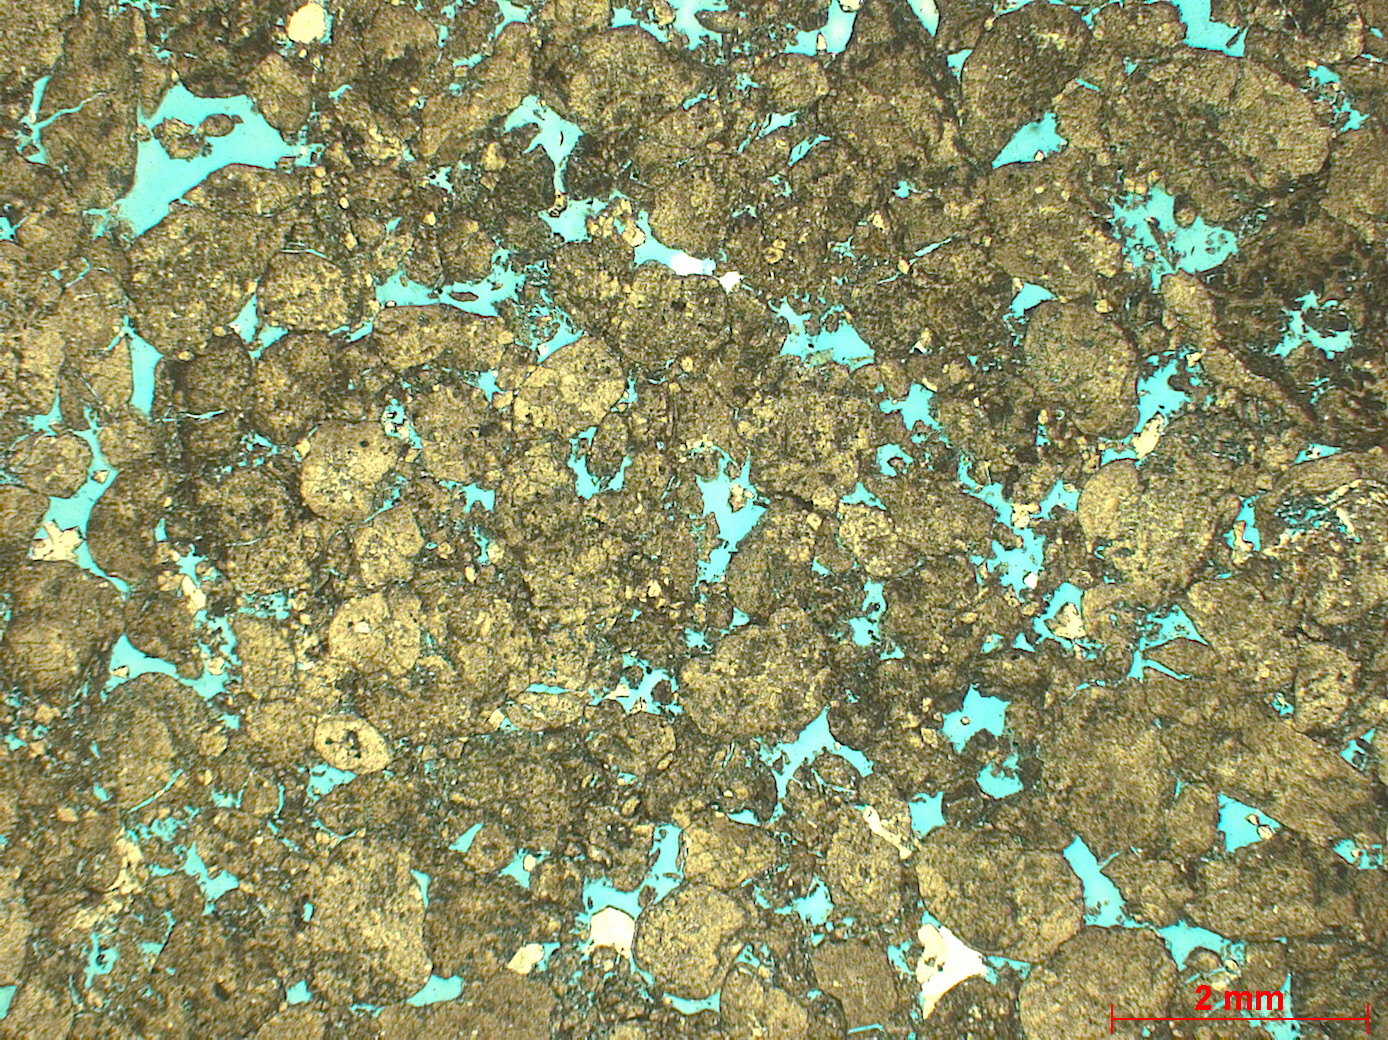
\includegraphics[width=\textwidth]{images/3-SPS-69_T04_5065,95_1,25x.jpg}
		\fonte{Sapinhoá project.}
	\end{minipage}
\end{figure}

Permeability, on the other hand, refers to the ease of passing liquids or gases through the porous space of the rock. It is measured in Darcy (D), with 1 D being equivalent to 1 $cm^3$ of fluid with a viscosity of 1 cP (centipoise) flowing through 1 $cm^2$ of a cross section of rock in 1 second under pressure of 1 atm/cm. As most rocks have an average permeability considerably less than 1 D, the measurement is usually made in mD (mili-Darcy) \cite{Buryakovsky2012}.

A common way used to measure the performance of carbonate rocks present in reservoirs is through mercury injection. This technique consists of forcing mercury with increasingly higher pressures into a rock sample. After that, a graph is generated relating the amount of pressure and the volume of injected mercury. From the graph, it is possible to visualize the conditions for, in real environments, the oil to be moved trough the rock \cite{Harbaugh1967}. In addition to being costly, this technique can also be destructive and permanently damage sample properties due to the amount of pressure required for laboratory testing.

Importantly, a rock can be highly porous and at the same time have a low permeability. This can happen if the pores have few connections between them (throats), making the fluids not easily pass through the rock \cite{Buryakovsky2012}.

\subsection{Artificial Intelligence}
Artificial Intelligence (AI) is an area with many practical applications and active research topics. Intelligent software are used to automate routine tasks, understand speech or images, make medical diagnoses and assist scientific research \cite{Goodfellow-et-al-2016}.

According to \cite{chollet2017deep}, it was long believed that with a sufficiently large and complex set of explicit rules to manage knowledge, it would be possible to achieve human-level AI. Although this form of programming manages to solve well-defined logical problems, other more complex problems, such as image classification, speech recognition and language translation, become unfeasible.

According to \cite{Goodfellow-et-al-2016}, for computers to behave in an intelligent way, it is not enough to solve formal problems consisting of a sequence of rules. It is necessary to capture the same knowledge of the world as human beings, a subjective and intuitive knowledge used in everyday life. Ironically, this knowledge that occurs naturally in the human mind is one of the biggest challenges in AI.

\subsection{Machine learning}
The difficulties faced by systems codified with formal knowledge and sets of rules suggest the need for AI systems to have the ability to acquire their own knowledge, through the extraction of raw data patterns. This ability is known as machine learning \cite{Goodfellow-et-al-2016}. \cite{mitchell1997machine} defined machine learning as follows: "A computer program is said to learn from experience \textit{E} with respect to some class of tasks \textit{T} and performance metrics \textit{ P}, if its performance at tasks in \textit{T}, as measured by \textit{P}, improves with experience \textit{E}."

In machine learning, computers are programmed to learn from past experience. For that, they employ a principle of inference called induction, in which generic conclusions are obtained from a particular set of examples. Thus, machine learning algorithms learn to induce a function or hypothesis capable of solving a problem from data that represent instances of the problem to be solved \cite{faceli2011}.

While in traditional programming a set of rules would be elaborated so that, along with a set of data, a processing is carried out and the answer obtained, in machine learning the processing is carried out based on the dataset combined with the results. From this combination, the algorithm is trained by calculating the hypothesis that maps each input data to the result. For this reason, the system is said to be trained rather than explicitly programmed \cite{chollet2017deep}. Figure~\ref{fig:progxml} demonstrates the difference between both paradigms.

\begin{figure}[h!]
	\caption{Comparative between traditional programming and machine learning}
	\label{fig:progxml}
	\centering%
	\begin{minipage}{.6\textwidth}
		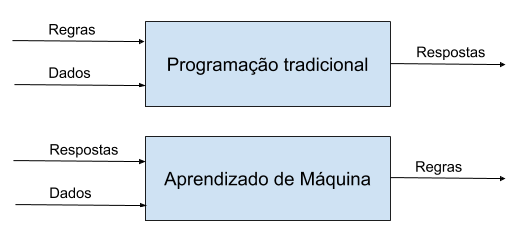
\includegraphics[width=\textwidth]{images/prog_ml.png}
		\fonte{Elaborated by the author based on \citeonline{chollet2017deep}.}
	\end{minipage}
\end{figure}

Algorithms trained rather than programmed tend to have advantages in complex problems because they don't rely on a lot of explicitly programmed rules to work as expected. Another benefit is flexibility to new examples. A model with good generalization does not depend on any manual changes or additional rules.

In relation to machine learning, deep learning seeks to solve problems with complex representations that a normal machine learning algorithm cannot efficiently solve. By learning in successive layers of increasingly significant representations, it manages to transform complex concepts into a sequence of simple concepts \cite{chollet2017deep}. Figure~\ref{fig:rel_deep} shows the relationship between the accuracy and the amount of data for machine learning approaches in contrast to deep learning, showing the improvement in accuracy as the amount of data increases.

\begin{figure}[h!]
	\caption{Relationship between the increase of accuracy and the amount of data}
	\label{fig:rel_deep}
	\centering%
	\begin{minipage}{.4\textwidth}
		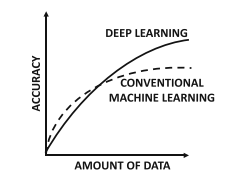
\includegraphics[width=\textwidth]{images/acc_deep_aggarwal.png}
		\fonte{\cite{aggarwal2018}.}
	\end{minipage}
\end{figure}

Just as machine learning is a subarea of AI, deep learning is a subarea of machine learning. The relationship between the three knowledge areas can be seen in Figure~\ref{fig:comparative}.

\begin{figure}[h!]
	\caption{Relationship between Artificial Intelligence, machine learning and deep learning}
	\label{fig:comparativo}
	\centering%
	\begin{minipage}{.5\textwidth}
		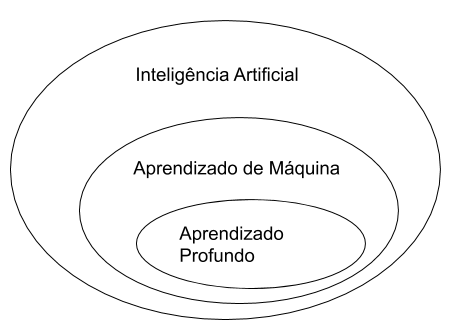
\includegraphics[width=\textwidth]{images/ai_ml_dl.png}
		\fonte{Elaborated by the author based on \citeonline{chollet2017deep}.}
	\end{minipage}
\end{figure}

According to \citeonline{russell2013artificial}, machine learning algorithms can be classified according to the relationship between a given input and that input's feedback, defining three main ways of learning by an intelligent agent:

\begin{itemize}
    \item \textbf{Supervised learning} - The agent observes input and output pairs and learns a function that maps input to output. Therefore, it depends on the data being already labeled with their respective outputs;
    \item \textbf{Unsupervised learning} - The agent learns patterns on inputs without any explicit feedback. Input data is not labeled as in supervised learning;
    \item \textbf{Reinforcement learning} - Sequential decision-making process, where the agent learns through a series of reinforcements, rewards and punishments received when interacting with the environment.
\end{itemize}

Machine learning tasks are also commonly divided according to different classes of problems that it tries to solve. According to \citeonline{mohri2018foundations}, they are:
\begin{itemize}
     \item \textbf{Classification} - Input data must be classified into some discrete numeric category, within a finite set of values. It can contain two categories (binary classification) or multiple categories (multiclass classification). Examples: Classification of images as being of a dog or cat (binary) and classification of images of handwritten characters (multiclass);
    \item \textbf{Regression} - Input data must be mapped to a continuous numeric value. Examples: Prediction of a stock's value on the stock market and prediction of a property's value;
    \item \textbf{Ranking} - Ordering items according to some criteria. Example: Determination of the most relevant documents and web pages in a web search;
    \item \textbf{Clustering} - Division of a set of items into smaller sets based on similarities. Example: Identification of common characteristics between different users of a virtual store;
    \item \textbf{Dimensional reduction} - Transformation of an initial representation of a set of items to a representation in less dimensions without losing important properties. Example: Pre-processing digital images for more complex deep learning tasks.
\end{itemize}

In this work, a training approach with supervised learning will be used to treat a regression problem. The data is labeled with the expected output for each of the inputs and the labels are part of a continuous set of values. 

\subsection{Artificial neural networks}
Artificial Neural Networks (ANN) were developed based on the functioning of the human brain, where its computational units are treated in an analogous way to biological neurons. They are theoretically able to learn any mathematical function from training on a sufficient set of data \cite{aggarwal2018}.

The neuron of an artificial neural network applies an activation function on the sum of a set of inputs multiplied by a set of weights and added to a constant, or bias. The result is propagated and becomes an input for the next neuron. This is the simplest form of an artificial neuron, being called a \textit{Perceptron} \cite{aggarwal2018}. In Figure~\ref{fig:perceptron} a neuron is being represented with the inputs (\textit{x\textsubscript{1}, x\textsubscript{2}, x\textsubscript{3}, x\textsubscript{4}, x\textsubscript{5}}), the weights (\textit{w\textsubscript{1}, w\textsubscript{2}, w\textsubscript{3}, w\textsubscript{4}, w\textsubscript{5}} ), the bias (\textit{b}) and the output (\textit{y}). A neural network is nothing more than a set of artificial neurons interconnected with multiple layers, as shown in Figure~\ref{fig:ann}. The first layer of the network is called the input layer, the last one is called the output layer and the other intermediate layers are called hidden layers. 

\begin{figure}[h!]
	\caption{Artificial neuron, or \textit{Perceptron}}
	\label{fig:perceptron}
	\centering%
	\begin{minipage}{.5\textwidth}
		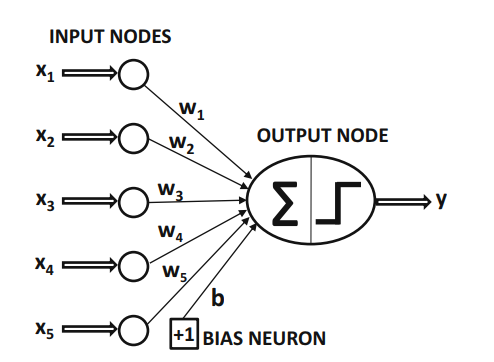
\includegraphics[width=\textwidth]{images/perceptron_aggarwal.png}
		\fonte{\cite{aggarwal2018}.}
	\end{minipage}
\end{figure}

\begin{figure}[h!]
	\caption{Artificial neural network}
	\label{fig:ann}
	\centering%
	\begin{minipage}{.8\textwidth}
		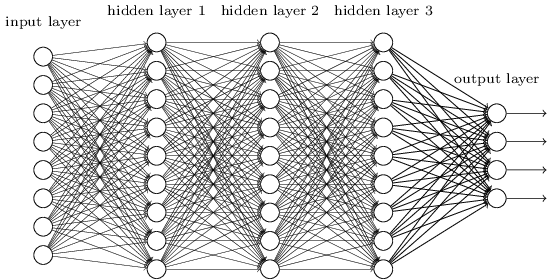
\includegraphics[width=\textwidth]{images/ann_nielsen.png}
		\fonte{\cite{nielsen2015neural}.}
	\end{minipage}
\end{figure}

\subsubsection{Gradient descent}
Gradient descent is a process applied during the training of a neural network to adjust its weights in order to find a global minimum value for the error function. From the calculation of the partial derivative of the error in relation to each of the weights, it is possible to determine whether the weight should increase or decrease \cite{heaton2015}.

The value of each step towards the minimum value is defined by a learning rate. This value should not be set too low, which could cause slow convergence, and not too high, which could cause a divergence from the global minimum value \cite{geron2019hands}.

In neural networks, a variation of the gradient descent algorithm called Stochastic Gradient Descent (SGD) is often used. It consists of applying gradient descent to small sets, or batches, of examples rather than the entire training set. This allows for a significant performance improvement, decreasing the network's training time \cite{LeCun2015deep}. Figure~\ref{fig:sgd} demonstrates the process of stochastic gradient descent seeking the smallest value for an error function.

In order to apply the gradient descent over all the weights of a neural network retroactively, the Backpropagation \cite{rumelhart1986learning} technique is used. Starting with the error value in the output, it can work in reverse from the final to the initial layers, updating the parameters with a technique called chain rule \cite{chollet2017deep}.

\begin{figure}[h!]
	\caption{Stochastic Gradient Descent}
	\label{fig:sgd}
	\centering%
	\begin{minipage}{.6\textwidth}
		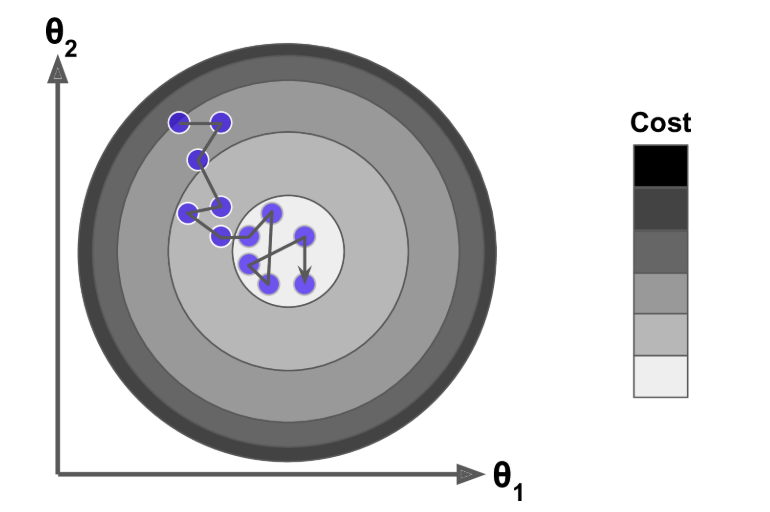
\includegraphics[width=\textwidth]{images/geron_sgd.png}
		\fonte{\cite{geron2019hands}.}
	\end{minipage}
\end{figure}

Two common problems related to gradient descent in neural networks are exploding gradient and vanishing gradient. They occur when gradients become extremely large or small to the point of harming or not influencing network training. Both cause problems during training, making it unstable and often making it impossible for the network to evolve during the process \cite{aggarwal2018, geron2019hands}.

\subsubsection{Overfitting and underfitting}
All models trained with machine learning can suffer from a problem called overfitting. This occurs when the model starts to perform well on training data but performs poorly on new data, so it cannot generalize. Some ways to avoid overfitting are: add more training data, regularization techniques and dropout layers. On the other hand, underfitting occurs when the model is not able to perform well even on the training data, so it is not able to optimize the training. One of the biggest challenges when designing a machine learning model is finding the sweet spot between being able to generalize over new data and optimizing the training data, avoiding both overfitting and underfitting \cite{chollet2017deep}.

\subsubsection{Loss Functions}
A loss function determines how different the expected result is from the result obtained by the neural network for each training sample. It is used in the calculation of the derivative for the adjustment of weights during training. It is also through loss functions that many of the performance evaluation metrics of a trained model are obtained \cite{heaton2015}. Therefore, choosing an appropriate loss function for the problem is very important to obtain good results.

The most used loss functions for regression problems are Mean Squared Error (MSE), and Mean Absolute Error (MAE). There is also a variation of the MSE called Root Mean Squared Error (RMSE), where a square root is applied to the result \cite{chai2014root}. Both are represented by the equations \ref{eq:mse} and \ref{eq:mae}, with $n$ being the number of samples, $\hat{y}$ the expected value and $y$ the value calculated by the model.

\begin{equation}
\label{eq:mse}
MSE = \frac{1}{n}\Sigma_{i=1}^{n}(\hat{y}_i - y_i)^2
\end{equation}

\begin{equation}
\label{eq:mae}
MAE = \frac{1}{n}\Sigma_{i=1}^{n}|\hat{y}_i - y_i|
\end{equation}
 
While the MAE function gives the same weight to all errors, the MSE function penalizes very large variations, giving greater weight to errors with larger absolute values \cite{chai2014root}. Thus, MAE becomes more suitable when errors are evenly distributed, while MSE becomes more suitable for normal distribution with the presence of some outliers \cite{chai2014root}.

As an alternative to the two functions, there is also the Huber loss function shown in equation~\ref{eq:huber}. This function is a hybrid of the two previous ones, enabling the behavior of the quadratic function and the absolute function according to the parameter $\delta$. It is considered a more robust function, being less prone and sensitive to noise in data \cite{Alqahtani2020, Holland1977}.

\begin{equation}
\label{eq:huber}
L_\delta(a) = \left\{\begin{array}{cc}\frac{1}{2}a^2& |a| \leq \delta\\ {}\delta(|a| - \frac{1}{2}\delta) & |a| > \delta\end{array}\right.
\end{equation}


\subsubsection{Activation functions}
Activation functions are used in artificial neural networks to transform an input value into an output value that is propagated to the next layer. They are necessary to prevent the output signal from having a linear format and to be able to map and train the model with more complex problems \cite{sharma2020}. Depending on the type of problem that is being tried to solve, different activation functions can be used. Also, each layer of the neural network can use a different activation function.

\paragraph{\textit{Sigmoid}}
Non-linear function that transforms the value to a range between 0 and 1, guaranteeing a small, positive value. It is generally used when the goal is to obtain a probability that an entry belongs to a certain category in binary classifications \cite{sharma2020}.

This type of function can cause a problem called vanishing gradient, when the gradient becomes so small and insignificant that it ends up not updating the weights, causing the entire network to not be trained.

\begin{equation}
\label{eq:sigmoid}
\sigma(x) = \frac{1}{1 + e^{-x}}
\end{equation}

\paragraph{Hyperbolic tangent (\textit{tanh})}
Very similar to the \textit{sigmoid} function, but generating values in the range between -1 and 1 and allowing negative values \cite{heaton2015}. It has the advantage that its gradient is not restricted to varying in just one (positive) direction \cite{sharma2020}. As with the \textit{sigmoid} function, it has the same vanishing gradient problem.

\begin{equation}
\label{eq:tanh}
tanh(x) = \frac{e^x - e^{-x}}{e^x + e^{-x}}
\end{equation}

\paragraph{Rectified Linear Unit (ReLU)}
One of the most used functions in neural networks, was proposed by \citeonline{nair2010} and solves the vanishing gradient problem. One of its biggest advantages is the fact that not all neurons are activated simultaneously. The neuron will be deactivated only when the function's output is zero. Due to this, it also manages to be more efficient than other functions \cite{sharma2020, nwankpa2018activation}.

One of the problems with this function is that neurons tend to die during training, causing the weights not to be updated and hindering the training \cite{nwankpa2018activation}.

There are also two simple variations of the ReLU function: the Leaked ReLU (LReLU) proposed by \citeonline{maas2013rectifier} to solve the neuron death problem and the Parameterized ReLU (PReLU) proposed by \citeonline{He_2015_ICCV}. The only difference between them is the value of $\alpha$, which assumes 0 in ReLU, 0.01 in LReLU and a parameterized value in PReLU.

\begin{equation}
\label{eq:relu}
ReLU(x) = \left\{\begin{array}{cc}x& x \geq 0\\ {}\alpha x& \mathrm{x<0}\end{array}\right.
\end{equation}

\paragraph{Exponencial Linear Unit (\textit{ELU})}
Another variation of the ReLU function, proposed by \citeonline{clevert2016fast}. It also uses a parameterized value for the slope of the negative values of \textit{x}, with the difference of using a logarithmic curve \cite{sharma2020}.

\begin{equation}
\label{eq:elu}
ELU(x) = \left\{\begin{array}{cc}x& x \geq 0\\ {}\alpha(exp(x) - 1)& \mathrm{x<0}\end{array}\right.
\end{equation}

\paragraph{Scale Exponencial Linear Unit (SELU)}
Variation of the ELU function that was introduced by \citeonline{klambauer2017selfnormalizing} with self-normalizing properties, since the mean and variance converge to zero. This function manages to avoid the vanishing and exploding gradient problems \cite{nwankpa2018activation}.

\begin{equation}
\label{eq:selu}
SELU(x) = \lambda\left\{\begin{array}{cc}x& x \geq 0\\ {}\alpha(exp(x) - \alpha)& \mathrm{x<0}\end{array}\right.
\end{equation}

Being $\alpha \approx 1.6733$ and $\lambda \approx 1.0507$.

\paragraph{\textit{Swish}}
Proposed by \citeonline{ramachandran2017searching}, it is a combination of the \textit{sigmoid} and ReLU functions. Like ReLU, it has an open upper limit and a closed lower limit, but it contains a smooth curve and is not monotomous. Its smoothness makes the function generate better optimization and generalization results when used in deep networks \cite{ramachandran2017searching, nwankpa2018activation}.

According to \citeonline{ramachandran2017searching}, the main advantages of the \textit{swish} function are its simplicity and high accuracy, since it does not suffer from the vanishing gradient problem and even so it achieves a good propagation of information during training.

\begin{equation}
\label{eq:swish}
swish(x) = x \cdot \sigma(x) = \frac{x}{1 + e^{-x}}
\end{equation}

\subsubsection{Metrics}
In addition to loss functions, which are also used as performance metrics, there are other measures often used in regression problems to measure model accuracy. These metrics do not influence training and are used to measure model performance. The coefficient of determination ($R^2$) is a metric commonly used to determine the predictive power of regression algorithms. It can be interpreted as the percentage of variance of the dependent variables that can be "explained" by the model. The closer to 1 (100\%) the value of $R^2$, the better the predictive capacity of the model on the dependent variables \cite{Erofeev2019, Nagelkerke1991YEAR}. It is defined by the equation~\ref{eq:r2}, with $\hat{y}_i$ being the real values, $y_i$ the values predicted by the model and $\overline{y}$ the mean of the values of $y$ :

\begin{equation}
\label{eq:r2}
R^2 = 1 - \frac{\sum_{i}(\hat{y}_i - {y}_i)^2}{\sum_{i}(\hat{y}_i - \overline{y})^2},
\end{equation}



\subsection{Convolutional neural networks}
Convolutional Neural Networks (CNN) \cite{LeCun1998} are designed to process input data in multi-vector format, representing a dependence of space or proximity between each input value. These vectors can be one-dimensional for temporal data such as signals and sequences, two-dimensional for images and audio spectrograms, or three-dimensional for video and volumetric images \cite{LeCun2015deep}. Its structure is very similar to artificial neural networks, with the difference that they use mathematical operations of convolution instead of simple matrix multiplication in at least one of its layers \cite{Goodfellow-et-al-2016}.

In addition to the convolutional layer, they can also have activation and pooling layers. Together, the layers transform the input data, inferring which characteristics are critical to the problem through the training process. For this, they also use the same techniques conventionally used in artificial neural networks: gradient descent and backpropagation. Figure~\ref{fig:cnn} demonstrates the convolutional neural network model proposed by \citeonline{LeCun1998} for classification of handwritten digits, being one of the precursors of this type of network.

\begin{figure}[h!]
	\caption{CNN proposed by \citeonline{LeCun1998}}
	\label{fig:cnn}
	\centering%
	\begin{minipage}{1\textwidth}
		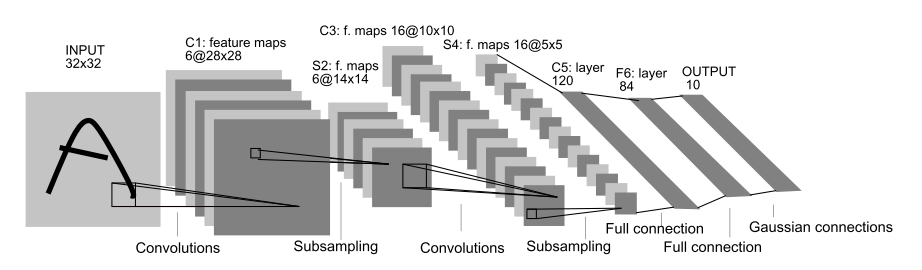
\includegraphics[width=\textwidth]{images/cnn_lecun.png}
		\fonte{\cite{LeCun1998}.}
	\end{minipage}
\end{figure}

\subsubsection{Convolutional layer}
In the convolutional layer, a convolution operation is performed on the input, performing calculations with multidimensional structures known as filters or kernels \cite{aggarwal2018}. These kernels are structures smaller than the input and are applied over sections of the same size and shifted until applied over the entire input.


The convolutional layer aims to highlight, in some way, the features that influence the final result of the network. While sorting animal images, for example, kernels could be adjusted to highlight features such as the animal's paws or tail. The kernel values are adjusted during gradient descent and backpropagation, that is, the network is able to identify by itself which features are most relevant to the problem it is solving. These features may be similar to the features that the human brain identifies, or they may be completely different. \cite{aggarwal2018, heaton2015}. In Figure~\ref{fig:conv}, an image of a dog is displayed before and after applying the convolution operation.

\begin{figure}[h!]
	\caption{Image of a dog before and after the convolution}
	\label{fig:conv}
	\centering%
	\begin{minipage}{0.7\textwidth}
		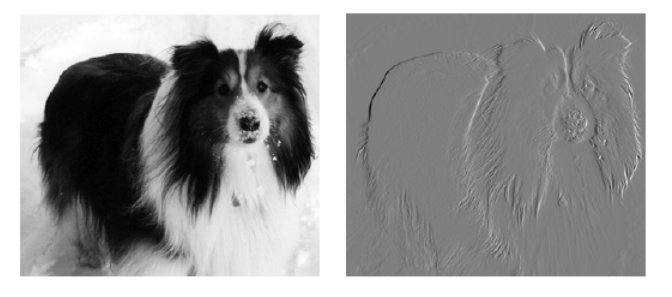
\includegraphics[width=\textwidth]{images/conv_goodfellow.png}
		\fonte{\cite{Goodfellow-et-al-2016}.}
	\end{minipage}
\end{figure}

\subsubsection{Activation layer}
The CNN's activation layer are very similar to activation layers in traditional neural networks, as they apply an activation function on the input. This operation does not affect the dimensionality of the input, being a one-to-one mapping. In convolutional networks, it is more common to use open activation functions such as ReLU or similar \cite{aggarwal2018}.

\subsubsection{Pooling layer}
The pooling layer reduces the dimensionality of the input according to some function. It is similar to convolution in that it performs operations on fractions of the input, with the difference that they do not have filters, so they are not affected during training, and in the output they generate reduced data. In addition to reducing overfitting, as they discard non-relevant information that could affect the output, they also reduce training time by decreasing the amount of data to be processed \cite{aggarwal2018}.

The most used type of pooling is max pooling, where for each window only the highest value is returned, as shown in Figure~\ref{fig:pooling}. There are others, like average pooling, which return the average of each window, but are not as used as max pooling. As the convolution layers highlight important features of the input, it just makes more sense to take the highest value rather than the average \cite{chollet2017deep}.

\begin{figure}[h!]
	\caption{Max pooling}
	\label{fig:pooling}
	\centering%
	\begin{minipage}{0.8\textwidth}
		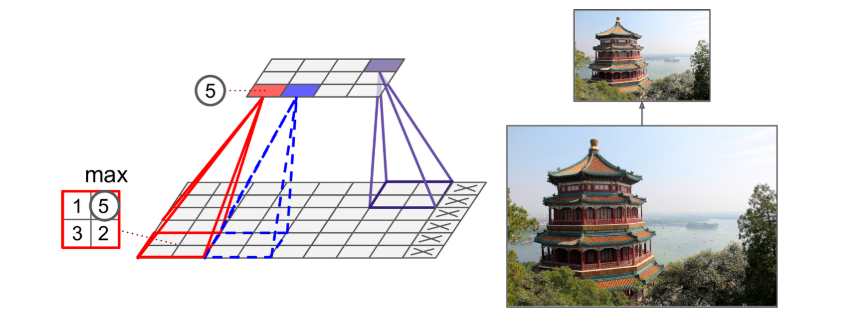
\includegraphics[width=\textwidth]{images/pooling_geron.png}
		\fonte{\cite{geron2019hands}.}
	\end{minipage}
\end{figure}

\subsubsection{Dense layer}
Dense layers are used at the end of convolutional networks and their behavior is also similar to artificial neural networks. After the spatial operations of the convolutional network, a flattening layer is applied to transform the multidimensional data into just one dimension, as expected by the dense layers \cite{aggarwal2018}.

\subsubsection{Dropout layer}
The dropout layer \cite{hinton2012improving} is applied over another dense layer and consists of randomly deactivating, or dropping, some percentage of neurons in the layer during training. The dropout percentage is usually between 20\% and 50\%. This technique is used to reduce overfitting, as it helps the network to adapt to noise in the input data, preventing it from becoming "hooked" on "perfect" data, which is generally not the case with real data \cite{chollet2017deep}.

%=======================================================================
% Trabalhos relacionados
%=======================================================================
\section{Related work}

To support this work and identify state of the art aspects in the identification of rock properties using AI, a non-systematic search was carried out in qualified journals, using research terms linked to the general theme addressed. Terms such as "porosity", "permeability", "carbonate rocks", "convolutional networks", "machine learning" and "deep learning" were used, filtering works in both Portuguese and English developed in the last 5 years. From the search results, the most relevant works with the highest number of citations were selected.

The vast majority of related works that identify rock properties using machine learning use a dataset of three-dimensional grayscale images collected using the x-ray computed microtomography technique. These are different data from those used in this work, but these works were kept for comparative purposes.

In the work of \citeonline{Sudakov2019}, a study was carried out on different machine learning techniques to predict permeability from digital rocks (3D images). In the end, they concluded that 3D convolutional networks bring the best results with an absolute mean error of 3.37\%, as they can identify complex features without losing space dependence in all three dimensions. This work ended up serving as a starting point and influencing several other works with similar themes.

\citeonline{bordignon2019deep} used synthetic data (set of spheres) to train a 3D convolutional neural network in order to predict the grain size and porosity distributions in an agile way. In the image pre-processing, a simple thresholding segmentation technique was used. Then, the trained model was applied to real samples of Berea sandstone. The solution converged to a low error, but the exact value was not described. The main contribution of the work was the fact that it used synthetic data to carry out the training, avoiding the need for image collection and annotation.

In the study of \citeonline{Alqahtani2020}, a convolutional network model was trained to predict porosity, specific surface area and mean pore size. Real data from three types of sandstone were used in 3D format and converted to 2D slices. The final average error obtained was considerably low, with a Hubber loss of 2.8\%, MSE of 4.5\% and MAE of 5.4\%. The $R^2$ obtained was 0.96 for porosity, 0.92 for specific surface area and 0.71 for average pore size. The good results demonstrate the potential for using convolutional networks on this type of task. A limitation of this work is that it depended on the application of segmentation techniques in its process in order to obtain good results. In addition, the permeability prediction was not performed, being indicated as future work.

\citeonline{Tembely2019} used a combination of traditional numerical techniques with machine learning techniques to predict permeability from thousands of 3D images. They obtained the best result using a deep neural network with a $R^2$ of 0.9156, but they did not get good results when using convolutional neural networks, both directly from the images and also using the physical properties of the rocks. Finally, it emphasizes the network's agility of prediction compared to traditional models for identifying the permeability of rocks.

\citeonline{Wu2018} proposed a convolutional neural network model to predict the permeability of rocks. They used a dataset of artificially generated 2D images together with physical rock data and, as well as \citeonline{bordignon2019deep}, applied the model to real images. An $R^2$ of 0.926315 and MSE of 0.000470 was obtained. The main focus of the work, according to the authors, is to serve as a proof of concept for the adoption of image recognition techniques from convolutional networks in predicting the permeability of real rocks, proving effective in this regard.

Meanwhile, \citeonline{Araya-Polo2018} sought to predict permeability with a convolutional network and 2D images collected from Scanning Electron Microscopy (SEM), another image collection technique that produces images at higher resolutions compared to X-ray microtomography, obtaining an average error of 11.69\% (MSE) and a $R^2$ of 0.7967 on the test data. The lack of a complete architecture that uses images collected with this technology is highlighted.

In general, there is a tendency to use convolutional architectures, based on their good results and adequacy to the needs of rock data treatment. It is also noticeable the growth and potential of using these networks for regression tasks, something that is not so common in relation to classification tasks and is bringing good results. In addition, the fact that convolutional networks are able to identify properties in a practical and fast way relates very well to current geological needs in search of better identification of rocks. Although this work is focused on the application of this architecture in carbonate rocks, found mainly in oil wells, its use can be easily extended to include different use cases as needed.

%=======================================================================
% Materiais e métodos
%=======================================================================
\section{Materials and methods}
The purpose of this work is to carry out experiments with a two-dimensional convolutional neural network, capable of identifying the porosity and permeability of rocks from images. In the next sections, the dataset used for training and validation, the structure of the elaborated network and all the pre-processing steps performed will be described in more detail.

\subsection{Dataset}
The dataset consists of images of petrographic slices obtained from rock samples collected at different depths during the drilling of well P02 in Petrobras Sapinhoá field, located in the Brazilian pre-salt. As can be seen in Figure~\ref{fig:campo_sapinhoa}, the Sapinhoá field has a total area of 233 $km^2$, being located in the central portion of the Santos Basin, approximately 360 km off the coast of the state from São Paulo and 290 km away from the city of Rio de Janeiro \cite{sapinhoa_anp}. The location of well P02 within the Sapinhoá field, as well as its depth, can be seen in Figure~\ref{fig:sapinhoa}.

\begin{figure}[h!]
	\caption{Location of the Petrobrás Sapinhoá field}
	\label{fig:campo_sapinhoa}
	\centering%
	\begin{minipage}{0.8\textwidth}
		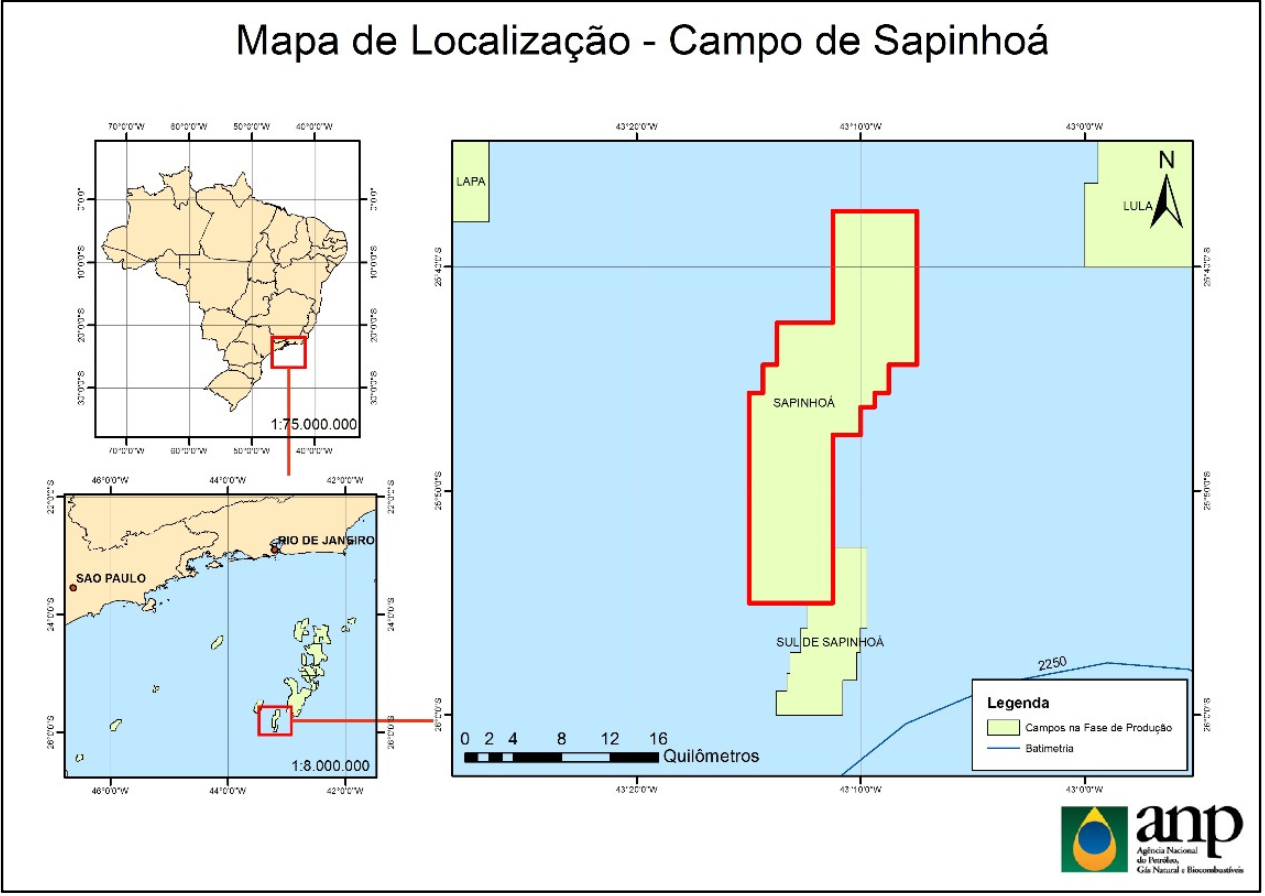
\includegraphics[width=\textwidth]{images/campo_sapinhoa.png}
		\fonte{\cite{sapinhoa_anp}}
	\end{minipage}
\end{figure}

\begin{figure}[h!]
	\caption{Location of well P02 in the Sapinhoá field}
	\label{fig:sapinhoa}
	\centering%
	\begin{minipage}{0.5\textwidth}
		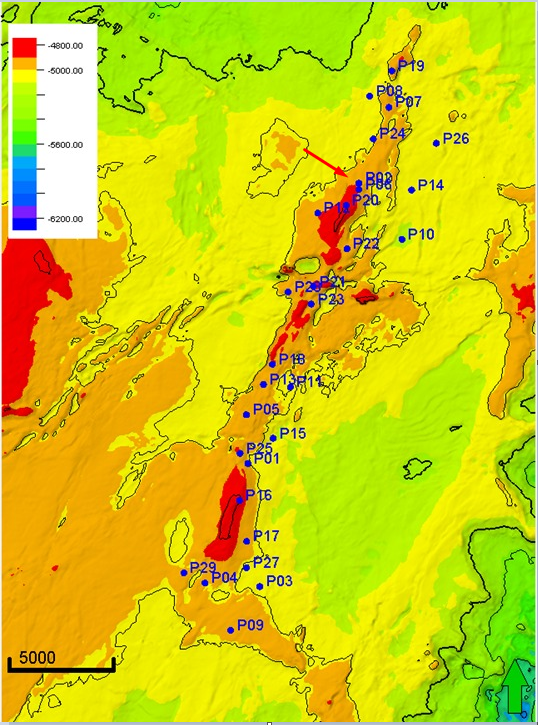
\includegraphics[width=\textwidth]{images/sapinhoa.png}
		\fonte{Sapinhoá project.}
	\end{minipage}
\end{figure}

The rock samples collected during the drilling of the well were then cut into a blade shape, representing a thin section, and later photographed in natural light with special equipment. The slides were provided by Petrobras, while the work of analyzing and photographing the samples was carried out by the research group of the Sapinhoá project. In Figure~\ref{fig:rocha-4987,05} one of these thin sections can be observed, where the pores can be distinguished from minerals through their bluer colors.


\begin{figure}[h!]
	\caption{Image of rock sample collected at a depth of 4987.05 m}
	\label{fig:rocha-4987,05}
	\centering%
	\begin{minipage}{0.5\textwidth}
		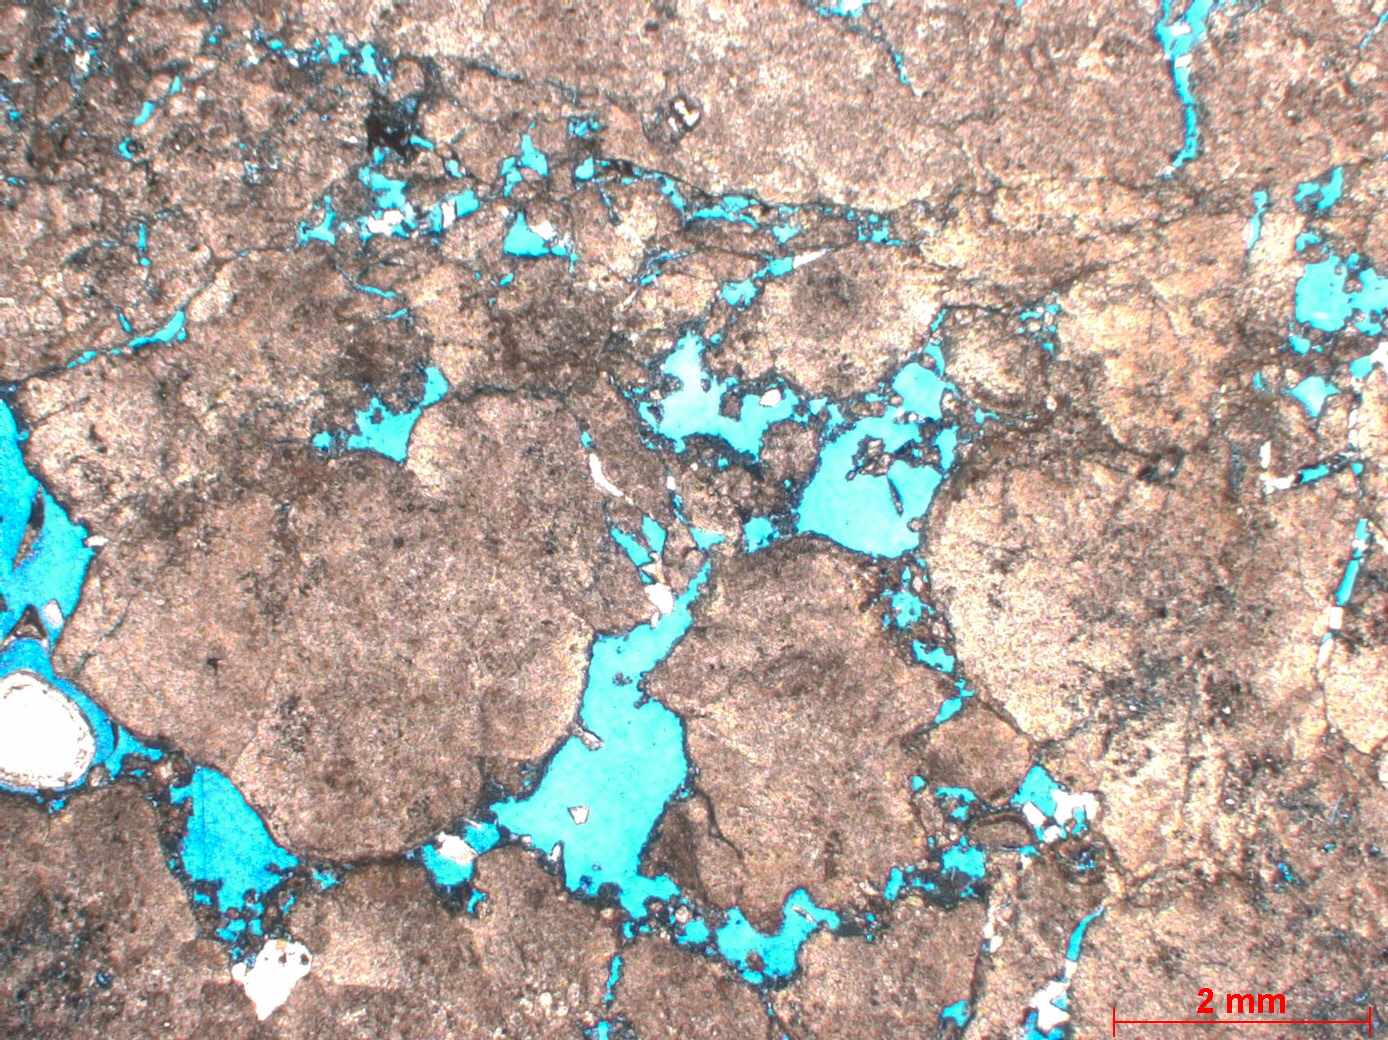
\includegraphics[width=\textwidth]{images/3-SPS-69_T01_4987,05_1,25x.jpg}
		\fonte{Sapinhoá project.}
	\end{minipage}
\end{figure}


As for the labels, porosity and permeability data obtained through the use of laboratory equipment and analysis by geology specialists were made available for each image. Figure~\ref{fig:poroxperm} shows a comparison between the porosity and permeability of each rock sample from the dataset. It is possible to notice that the permeability data are slightly unbalanced, with few samples having permeability above 2000 mD. The porosity data are more evenly distributed, having a lot of both low and high porosity samples. Another information that can be extracted from Figure~\ref{fig:poroxperm} is the lack of a direct relationship between porosity and permeability. A high porosity does not mean that the rock will have good permeability. There are samples with high porosity and low permeability, as the pores may not be connected to each other.

\begin{figure}[h!]
	\caption{Comparison between porosity and permeability of each rock sample}
	\label{fig:poroxperm}
	\centering%
	\begin{minipage}{0.5\textwidth}
		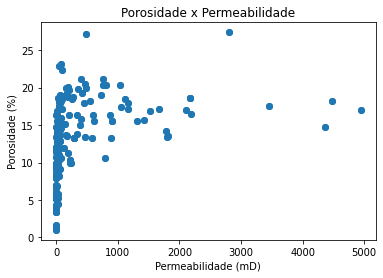
\includegraphics[width=\textwidth]{images/poroxperm.png}
		\fonte{Elaborated by the author.}
	\end{minipage}
\end{figure}

\subsection{Data preparation}
183 images with resolutions of 1388x1040 and 1384x1036 pixels were used, each one representing a sample of rock collected at different depth of the well. The 183 images were resized to a standard resolution of 1384x1036 pixels, keeping them close to the original resolution and preventing loss of information. Subsequently, all images were mirrored in order to generate new samples for better training of the network, generating a total of 366 images for training, validation and testing. It is important to emphasize that image mirroring does not affect the identification of porosity or permeability, that is, both properties remain the same regardless of the viewing angle.

From the 366 images, a random division of 70\% for training, 15\% for validation and 15\% for testing was performed. While training data is used to adjust network parameters, validation data is used during training to measure the quality and improvement of metrics on new data during training. Test data, on the other hand, are used after the end of network training, as a way to measure the quality of generalization of the model with data without any influence on training.

The next step was to change the scale of the images, as they were in RGB format, containing three values from 0 to 255 corresponding to red, green and blue color level. All values were divided by 255, resulting in values between 0 and 1 and maintaining the same distance relationship between them without losing information. The same was done for the labels: the porosity was divided by 100 to transform the percentage values, from 0 to 100, into decimal values between 0 and 1 and the permeability was divided by 1000 to convert the mD values (0 to 5000) to D (0 to 5). This is important to streamline neural network training and help avoid issues such as vanishing and exploding gradient.

\subsection{Model}
The model was developed using the Python programming language, using the Keras framework \cite{chollet2015keras} together with TensorFlow \cite{abadi2016tensorflow}. It consists of convolutional layers of 128, 64 and 32 neurons with ReLU activation function together with layers of max pooling and dropout (Table~\ref{tab:model_cnn}). The model was developed based on the structure of models found in the state of the art and adapted so that the results were the best possible with the data used. Some of the changes made were the addition of convolutional layers, with different number of neurons, and max pooling layers. Other models were experimented with, with different activation functions, layers and number of neurons, but none obtained better results than the one presented.

Furthermore, experiments were also carried out with segmentation techniques using unsupervised learning and applied to the images before moving to the convolutional network, but there was no noticeable difference in the results and it added a high computational cost, considerably increasing the total execution time. It is believed that there was no improvement due to the fact that the images already have a high contrast difference between pore and mineral. For these reasons, the application of this technique on the model was not continued, and the images were used in the convolutional network in its original form.
 
\begin{table}[h!]
	\caption{Proposed convolutional neural network model}
	\label{tab:modelo_cnn}
	\centering%
	\begin{minipage}{.6\textwidth}
		\begin{tabular*}{\textwidth}{llll}
			\hline
			\textbf{Layer} & \textbf{Neurons} & \textbf{Activation} & \textbf{Kernel}\\
			\hline
			Convolutional & 32 & ReLU & 3x3\\
			Max Pooling & - & - & 2x2\\
			Convolutional & 32 & ReLU & 3x3\\
			Max Pooling & - & - & 2x2\\
			Convolutional & 64 & ReLU & 3x3\\
			Max Pooling & - & - & 2x2\\
			Convolutional & 64 & ReLU & 3x3\\
			Max Pooling & - & - & 2x2\\
			Convolutional & 128 & ReLU & 3x3\\
			Max Pooling & - & - & 2x2\\
			Convolutional & 128 & ReLU & 3x3\\
			Max Pooling & - & - & 2x2\\
			Dropout & - & - & 20\%\\
			Dense & 64 & ReLU & -\\
			Dense & 32 & ReLU & -\\
			Dense & 1 & Identity & -\\
			\hline
			\textbf{Total parameters:} & \textbf{3.352.993}\\
			\hline
		\end{tabular*}
		\fonte{Elaborated by the author.}
	\end{minipage}
\end{table}

The loss function used was the Huber function in conjunction with the Adam optimization algorithm \cite{kingma2017adam}. This algorithm is responsible for updating the weights of each layer of the network through the stochastic gradient descent. An advantage of Adam is its ability to adapt the learning rate according to the improvement in accuracy of the model \cite{kingma2017adam}.

The model was trained using a GPU environment with 25 GB of RAM memory provided by Google Colab over a maximum of 150 epochs (iterations across the entire training set). To avoid memory depletion, the parameter batch size was reduced, which indicates the number of training samples that are propagated by the network in each iteration, from 32 to 16. Thus, 16 iterations were needed in each epoch to propagate all training samples. The early stopping technique was also used so that the model stops training when it does not identify an improvement in the result, in order to avoid overfitting. The early stopping has been configured to monitor the loss function on the validation data with a patience of 20 epochs (periods followed without improvement in the metric being evaluated) and reset the network weights on activation. Thus, it guarantees that the final model will be trained with the best possible result obtained during training.

The same model was trained twice separately for porosity and permeability, resulting in two instances trained for each of the properties, as shown in Figure~\ref{fig:model}. Experiments were carried out using the same model to return the two properties together, but the results were considerably inferior to the proposed format.

\begin{figure}[h!]
	\caption{Proposed model structure}
	\label{fig:modelo}
	\centering%
	\begin{minipage}{0.7\textwidth}
		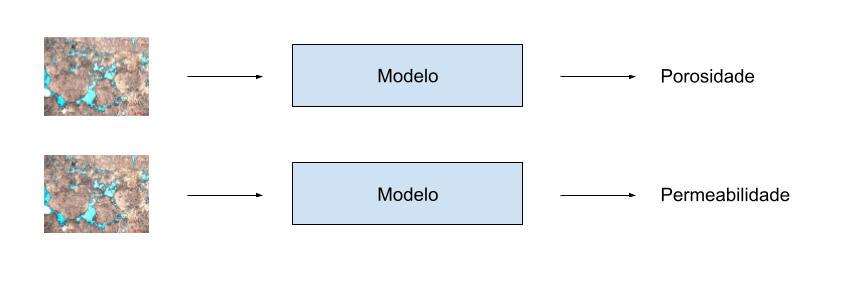
\includegraphics[width=\textwidth]{images/estrutura_modelo_cnn.png}
	\end{minipage}
    \fonte{Elaborated by the author.}
\end{figure}
%=======================================================================
% Resultados
%=======================================================================
\section{Results}

The metrics were obtained from the average of 5 training sessions, so that the results are more consistent and reliable. The metrics used were $R^2$, MAE, MSE and RMSE.

For porosity, an $R^2$ of 0.8385, MAE of 0.0132, MSE of 0.0004 and RMSE of 0.0209 was obtained. For permeability, an $R^2$ of 0.9826, MAE of 0.0700, MSE of 0.0161 and RMSE of 0.1256 was obtained. These data are consolidated in Table~\ref{tab:metrics}.

\begin{table}[h!]
	\caption{Metrics obtained through training}
	\label{tab:metrics}
	\centering%
	\begin{minipage}{.9\textwidth}
		\begin{tabular*}{\textwidth}{l|llll|llll}
			\hline
		    & \multicolumn{4}{c|}{\textbf{Porosity}} &  \multicolumn{4}{c}{\textbf{Permeability}}\\
			\hline
			\textbf{Training} & \textbf{$R^2$} & \textbf{MAE} & \textbf{MSE} & \textbf{RMSE} & \textbf{$R^2$} & \textbf{MAE} & \textbf{MSE} & \textbf{RMSE}\\
			\hline
			1 & 0.8487 & 0.0125 & 0.0004 & 0.0203 & 0.9814 & 0.0772 & 0.0173 & 0.1314\\
            2 & 0.8409 & 0.0138 & 0.0004 & 0.0208 & 0.9809 & 0.0661 & 0.0178 & 0.1334\\
            3 & 0.8041 & 0.0138	& 0.0005 & 0.0231 & 0.9743 & 0.0722	& 0.0239 & 0.1545\\
            4 & 0.8283 & 0.0135	& 0.0005 & 0.0216 & 0.9889 & 0.0618	& 0.0103 & 0.1014\\
            5 & 0.8704 & 0.0124 & 0.0004 & 0.0188 & 0.9876 & 0.0727	& 0.0115 & 0.1072\\
			\hline
			\textbf{Mean} & \textbf{0.8385} & \textbf{0.0132} & \textbf{0.0004} & \textbf{0.0209} & \textbf{0.9826} & \textbf{0.0700} & \textbf{0.0161} & \textbf{0.1256}\\
			\hline
		\end{tabular*}
		\fonte{Elaborated by the author.}
	\end{minipage}
\end{table}


Despite permeability being a much more complex property to be evaluated in relation to porosity, the model ended up obtaining a higher coefficient of determination, even with higher errors. This can be explained by the fact that the coefficient of determination uses the average of the output values in its calculation. Permeability has values between 0 D and 5 D, that is, the metric is much less penalized by small differences between the actual value and the predicted value. Meanwhile, for porosity they are percentage values between 0 and 1, resulting in a greater penalty for any small difference in the value predicted by the model.

Figure~\ref{fig:history} shows the evolution of the loss function over the epochs during one of the porosity and permeability trainings, both from the training data and from the validation data, until the stop due to the early stopping, when it has been detected that the error has stopped reducing after 20 epochs. Figure~\ref{fig:scatter} shows, respectively, the porosity and permeability predicted by the model in the test data in relation to the actual porosity of the rocks after one of the trainings.


\begin{figure}[h!]
	\caption{Evolution of the loss function over training epochs}
	\label{fig:history}
	\centering%
	\begin{minipage}{0.45\textwidth}
		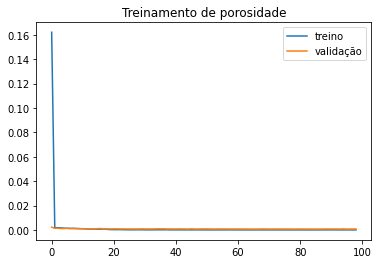
\includegraphics[width=\textwidth]{images/poro_train.png}
	\end{minipage}
	\begin{minipage}{0.45\textwidth}
		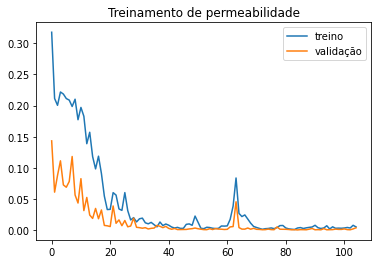
\includegraphics[width=\textwidth]{images/perm_train.png}
	\end{minipage}	
    \fonte{Elaborated by the author.}
\end{figure}

\begin{figure}[h!]
	\caption{Porosity predicted by the model in contrast to the actual porosity of the rocks}
	\label{fig:scatter}
	\centering%
	\begin{minipage}{0.45\textwidth}
		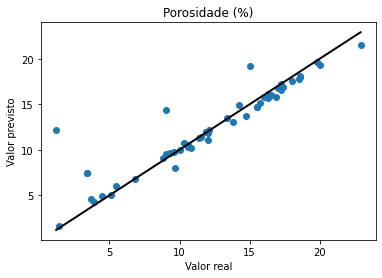
\includegraphics[width=\textwidth]{images/poro.png}
	\end{minipage}
	\begin{minipage}{0.45\textwidth}
		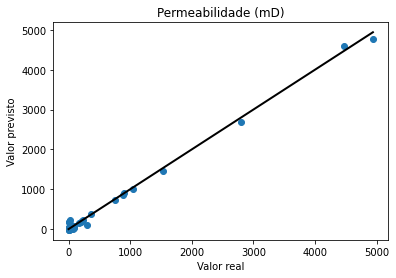
\includegraphics[width=\textwidth]{images/perm.png}
	\end{minipage}
    \fonte{Elaborated by the author.}
\end{figure}

In Figure~\ref{fig:scatter} it is possible to notice the presence of some outliers, mainly in the graph referring to the porosity prediction model. The most evident outliers were identified by the network with greater porosity than reality. Some of these samples can be seen in Figure~\ref{fig:outliers}, while in Figure~\ref{fig:normals} samples can be seen with a greater amount of hue found in the dataset. Compared to the other samples, it is possible to identify that there is a big difference in the shades of the colors, especially the mineral. One possible interpretation is that this may have confused the network, which may have interpreted parts of the mineral as being pores. Perhaps a way to mitigate this in the future is to add more samples with similar hue, such as some less common rock type that appears in smaller amounts in the dataset provided.

\begin{figure}[h!]
	\caption{Samples with the worst result on porosity prediction (outliers)}
	\label{fig:outliers}
	\centering%
	\begin{minipage}{0.4\textwidth}
		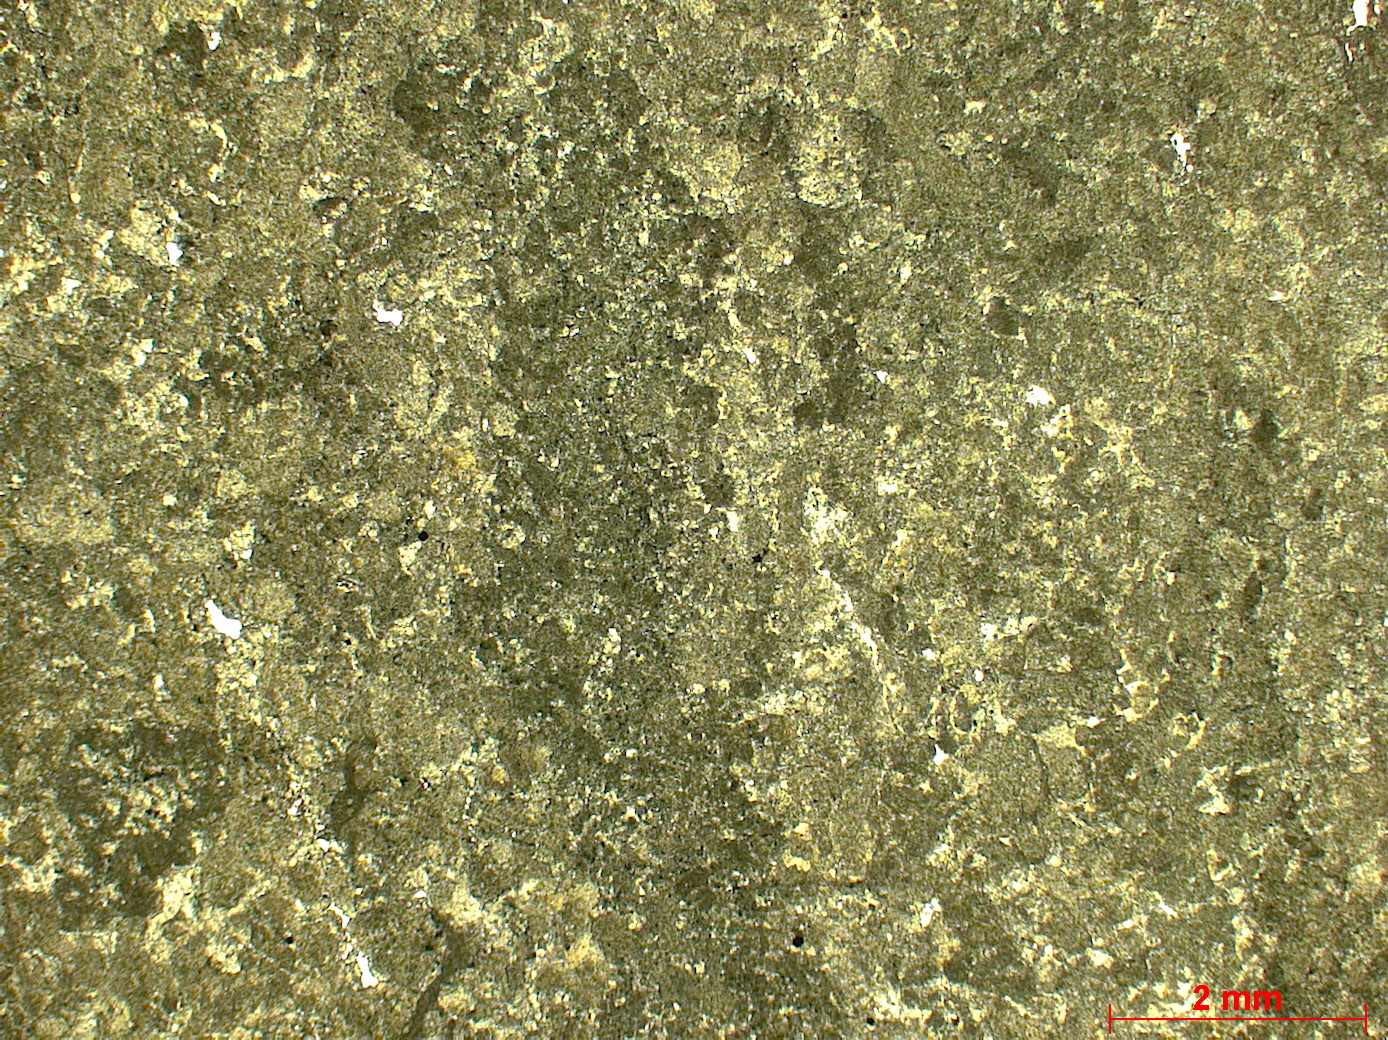
\includegraphics[width=\textwidth]{images/outlier_1.jpg}
	\end{minipage}
	\begin{minipage}{0.4\textwidth}
		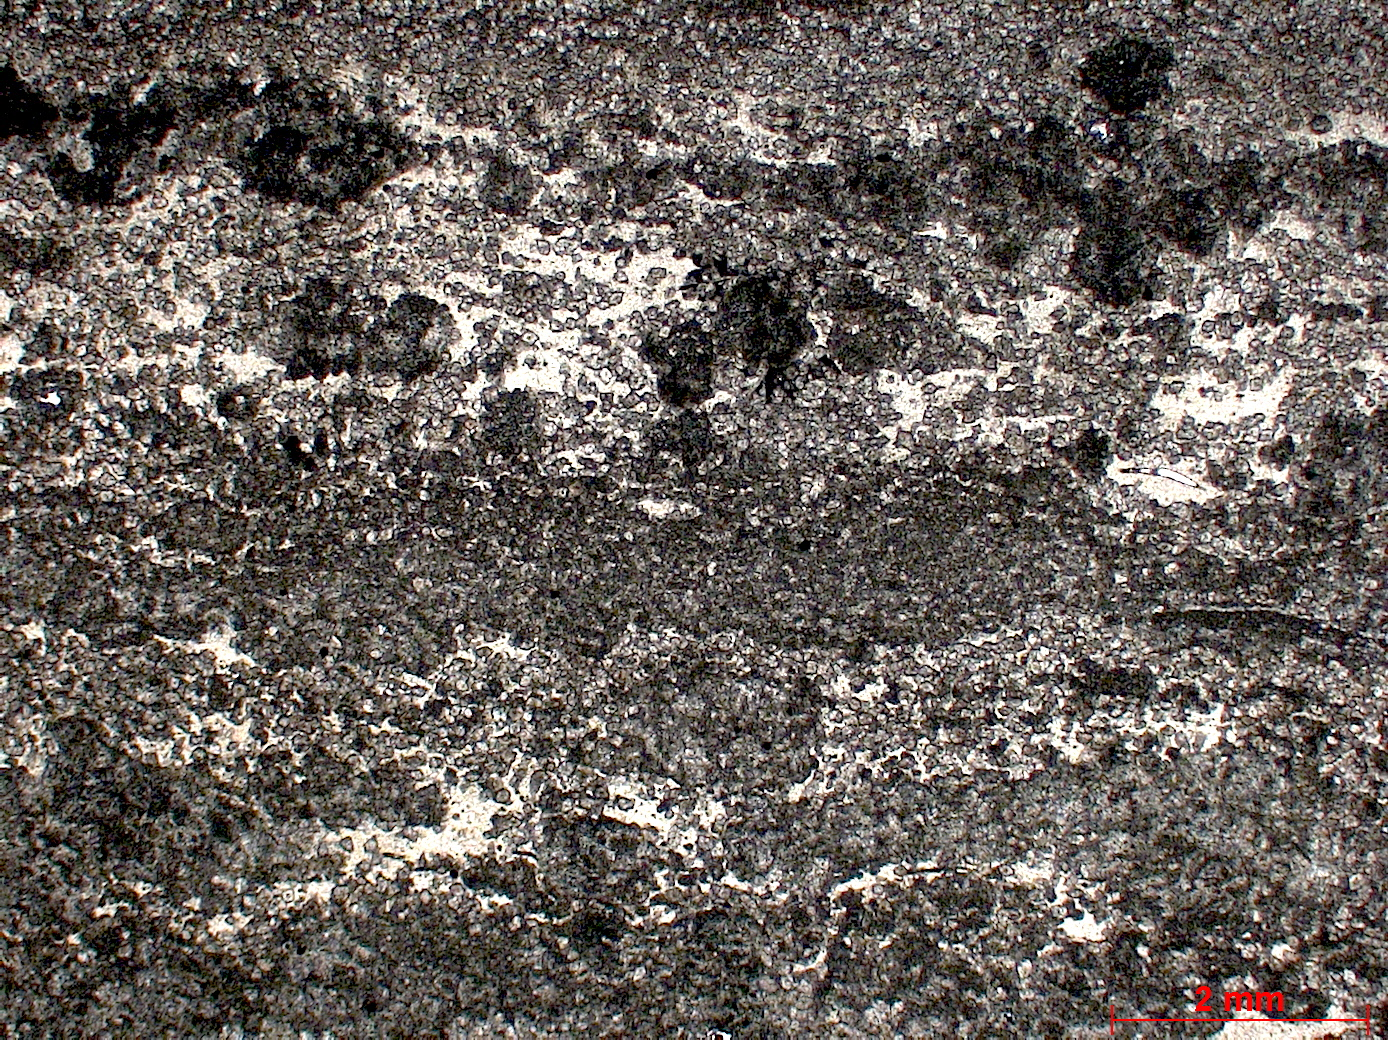
\includegraphics[width=\textwidth]{images/outlier_2.jpg}
	\end{minipage}
    \fonte{Sapinhoá project.}
\end{figure}

\begin{figure}[h!]
	\caption{Examples of samples found in most of the dataset}
	\label{fig:normals}
	\centering%
	\begin{minipage}{0.3\textwidth}
		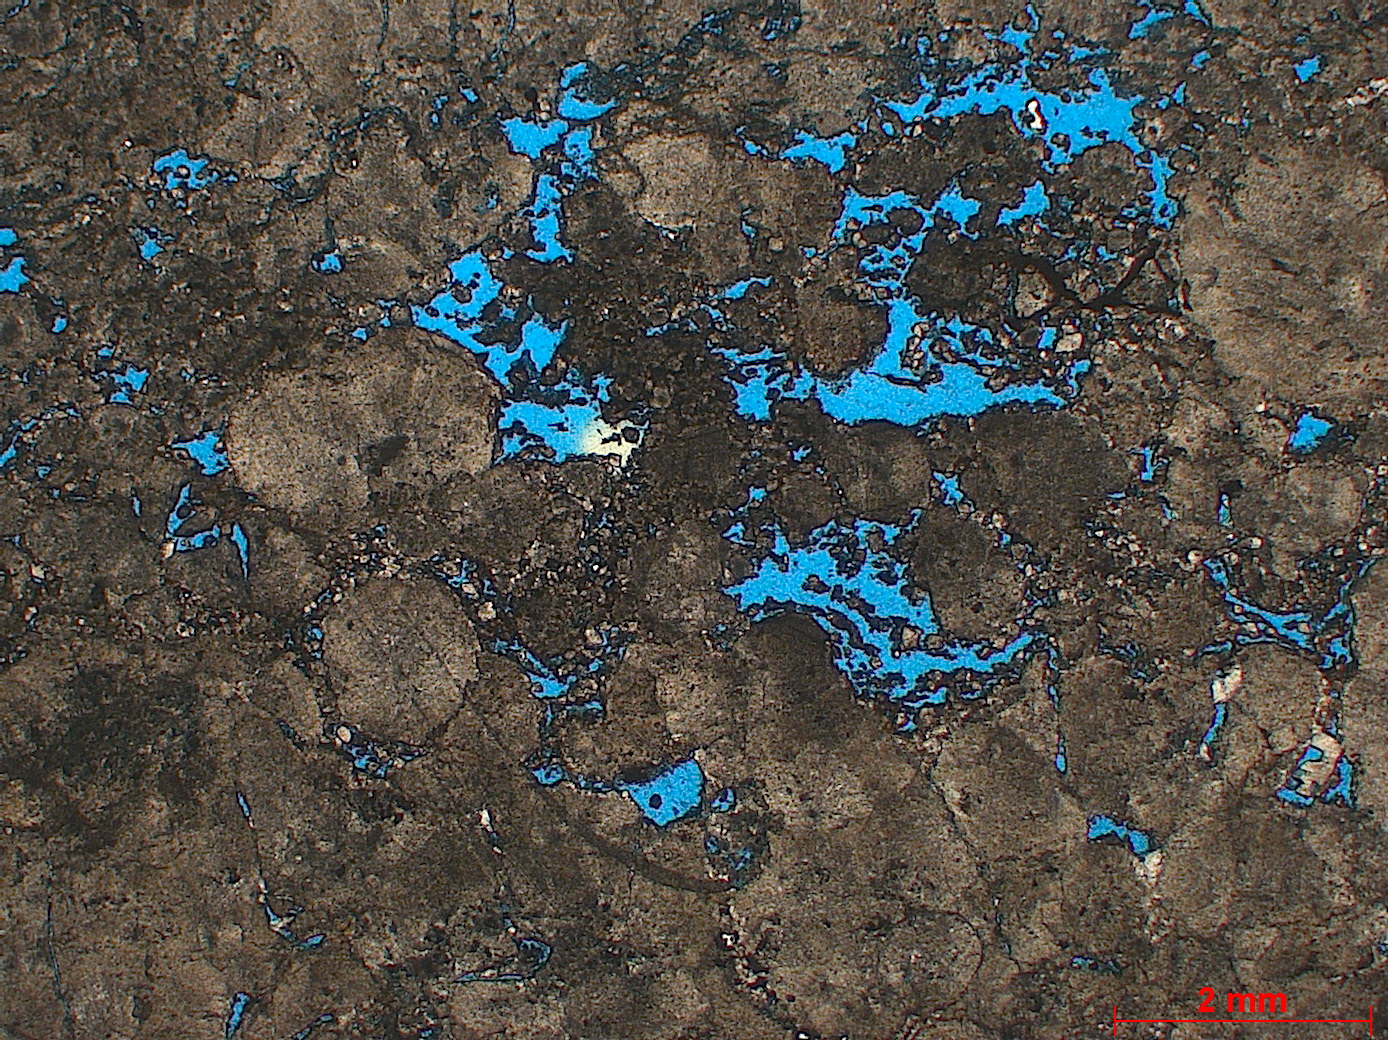
\includegraphics[width=\textwidth]{images/3-SPS-69_T01_4987,95_1,25x.jpg}
	\end{minipage}
	\begin{minipage}{0.3\textwidth}
		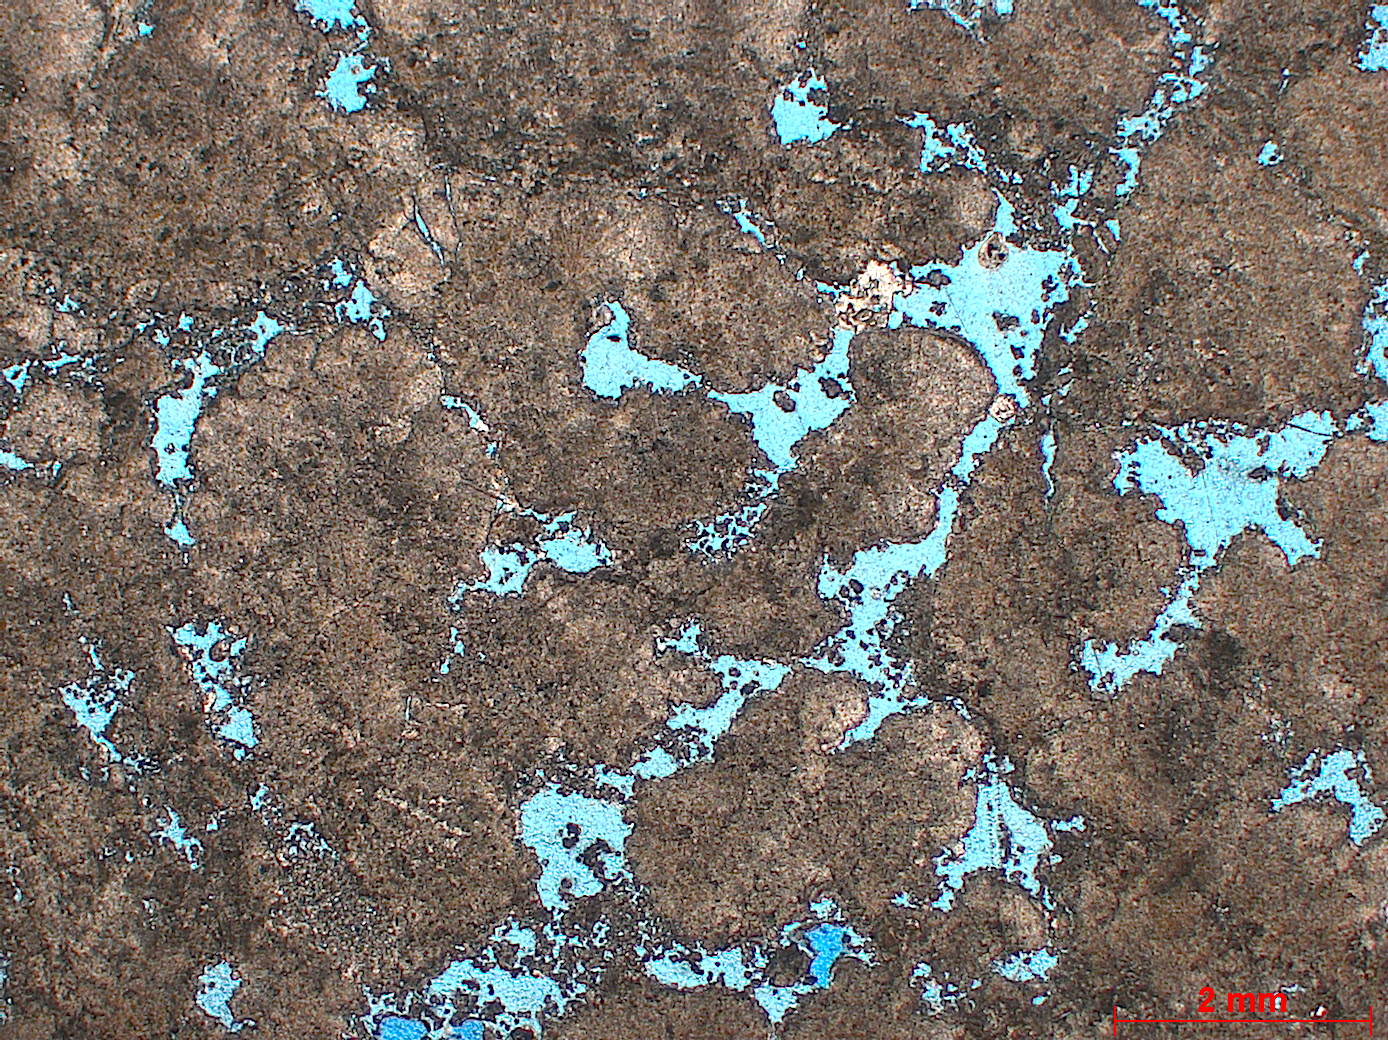
\includegraphics[width=\textwidth]{images/3-SPS-69_T01_4988,95_1,25x.jpg}
	\end{minipage}
	\begin{minipage}{0.3\textwidth}
		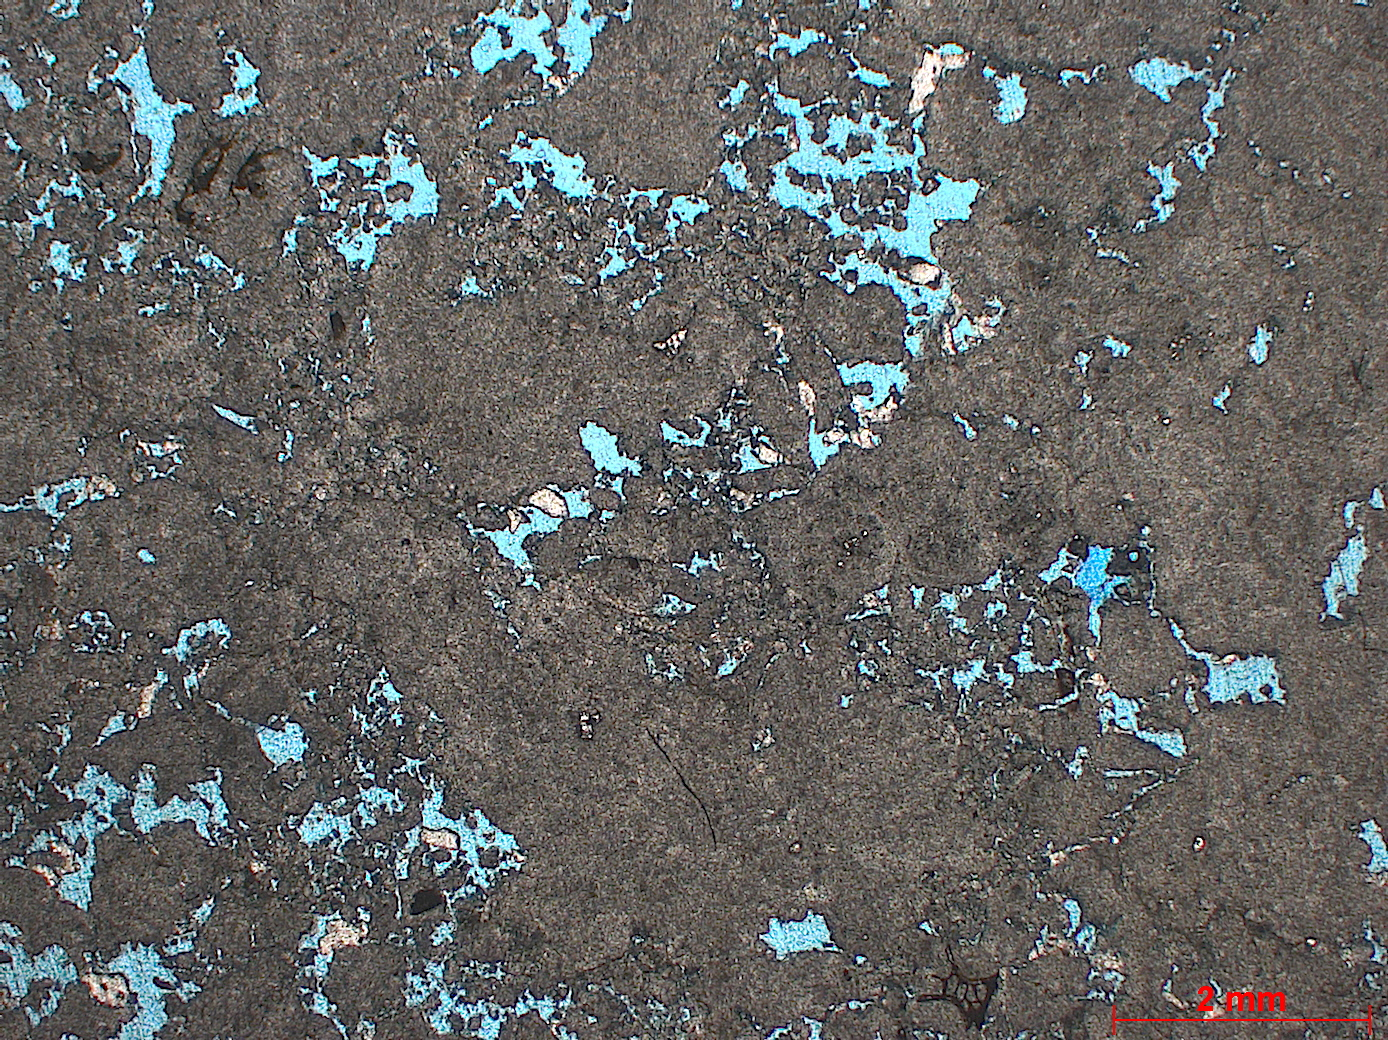
\includegraphics[width=\textwidth]{images/3-SPS-69_T01_4994,85_1,25x.jpg}
	\end{minipage}
    \fonte{Sapinhoá project.}
\end{figure}

As for the permeability graph, even though the data is unbalanced and the vast majority of samples have low permeability, the network managed to predict with good accuracy the few samples that had greater permeability. This is very important to help specialists make decisions and identify the oil wells with the highest extraction rate.

For comparison purposes, the work of \citeonline{Alqahtani2020} obtained a $R^2$ of 0.96 when measuring porosity from already segmented images and a $R^2$ of 0.78 from the original images in grayscale. The work of \citeonline{Wu2018} had a maximum $R^2$ of 0.878642 and an MSE of 0.001076. The work of \citeonline{Tembely2019} obtained a $R^2$ of 0.9156 in its neural network proposal. Although it is not possible to make a direct comparison between the works as they use different datasets, it is clear that the results of this work are positive as it obtained similar results with related works considered as state of the art in the area.

%=======================================================================
% Conclusões e Trabalhos Futuros
%=======================================================================
\section{Conclusion and future work}
This work aimed to apply machine learning, more specifically convolutional neural networks, to predict the porosity and permeability of carbonate rocks from images of samples collected during the drilling of an oil well. After an introduction to the problem and presentation of the theoretical concepts behind the work, related works were presented, the dataset used was detailed and the model was presented with all the pre-processing steps performed. Finally, the results obtained were presented, with a brief comparison with some related works, from which it appears that the results are similar to the results reported in the state of the art. It is important to emphasize that it is not possible to carry out a direct comparison between the works, but only in an informative way, as they do not use the same dataset. This implementation was a first step towards a more complete prediction model that has greater precision and is able to identify other more complex material properties, which may also be important for geology.

From the research and the results, it was possible to conclude that the use of convolutional neural networks can be very useful in predicting the properties of porous materials. The differential is the possibility of quick identification, without laboratory costs and human bias. As a result, it assists specialists in identifying the highest quality extraction wells that can bring more benefits when being explored.

As for the limitations of the work, the need for annotated data for training, the dependence on collection and photography of the thin sections, the sensitivity to outliers and also the fact of having few images, which may have harmed the results, can be highlighted.

One of the biggest challenges encountered during development was undoubtedly memory consumption. Due to the quantity and resolution of the images, depending on the structure of the network, it was not possible to carry out the training with the amount of memory available. Some techniques could be explored to reduce memory consumption, but at that time it was decided to use the images in their original format to avoid losing important information for training the network.

As future work, techniques can be studied to improve the results obtained, in addition to predicting more complex characteristics of rocks and pores, such as the number of gorges, types of pores or even the lithology of the rocks. The application of this model in other types of rocks (non-carbonate) can also be tried.

Some artificial intelligence techniques that can be tried are the use of cross validation and other data augmentation methods to generate new samples. Another possibility would be a study of segmentation techniques that could be applied before training to try to improve results.

Another factor that could improve the results is the use of more advanced techniques for collecting images of rocks in three dimensions, such as computerized x-ray microtomography. This technique has grown considerably in the oil industry in recent years \cite{Blunt2013, Andra2013a, Berg2017} as it represents the structure of the rock more completely and faithfully to reality in relation to two-dimensional images. Three-dimensional convolutional networks and segmentation techniques in the encoder-decoder format are some of the possibilities that can be explored and applied to these images, including as done in the works of \citeonline{Alqahtani2020, Karimpouli2019, ArRushood2020, DaWang2020}.









Examples of citations:

\cite{gomez1990isim3d, pebesma2004multivariable, hansen2018multiple}

Examples of citations in parentheses: 

\citep{gomez1990isim3d, pebesma2004multivariable, hansen2018multiple}

\section{Methodology}

This section includes an example of equation. 
 
\begin{equation}
\label{eqn:linear}
    y=ax+b.
\end{equation}


\subsection{Subsection}

This section contains another example of equation, different from Eq.  \ref{eqn:linear}.

\begin{equation} 
\label{eqn:quadratic}
    y=ax^2+bx+c
\end{equation}

\section{Algorithm and implementation}

Example of algorithm:
\begin{algorithm}
  \caption{Algorithm example }
  
  \begin{algorithmic}
  \label{alg:Alg1}
  \State \textbf{Input:} ...
   \newline

 \Statex \textit{1.} Step1
  \Statex \textit{2.} Step2;
 \State \textit{3.}  Step3;
  \newline
   \For{ i = 1,..., m}
   \State \textit{4.} Step 4;
    \For{ j = 2,..., n} 
   \State \textit{5.}  Step 5;
   \State \textit{6.} Step 6;
   \EndFor
  \EndFor 
  \newline
\State  \textbf{Output: } ... 
  \end{algorithmic} 
\end{algorithm} 


\section{Results}


This section includes an example of figure (Figure \ref{fig:Figure1}), from  \cite{de2021direct}.

\begin{figure}
\centering
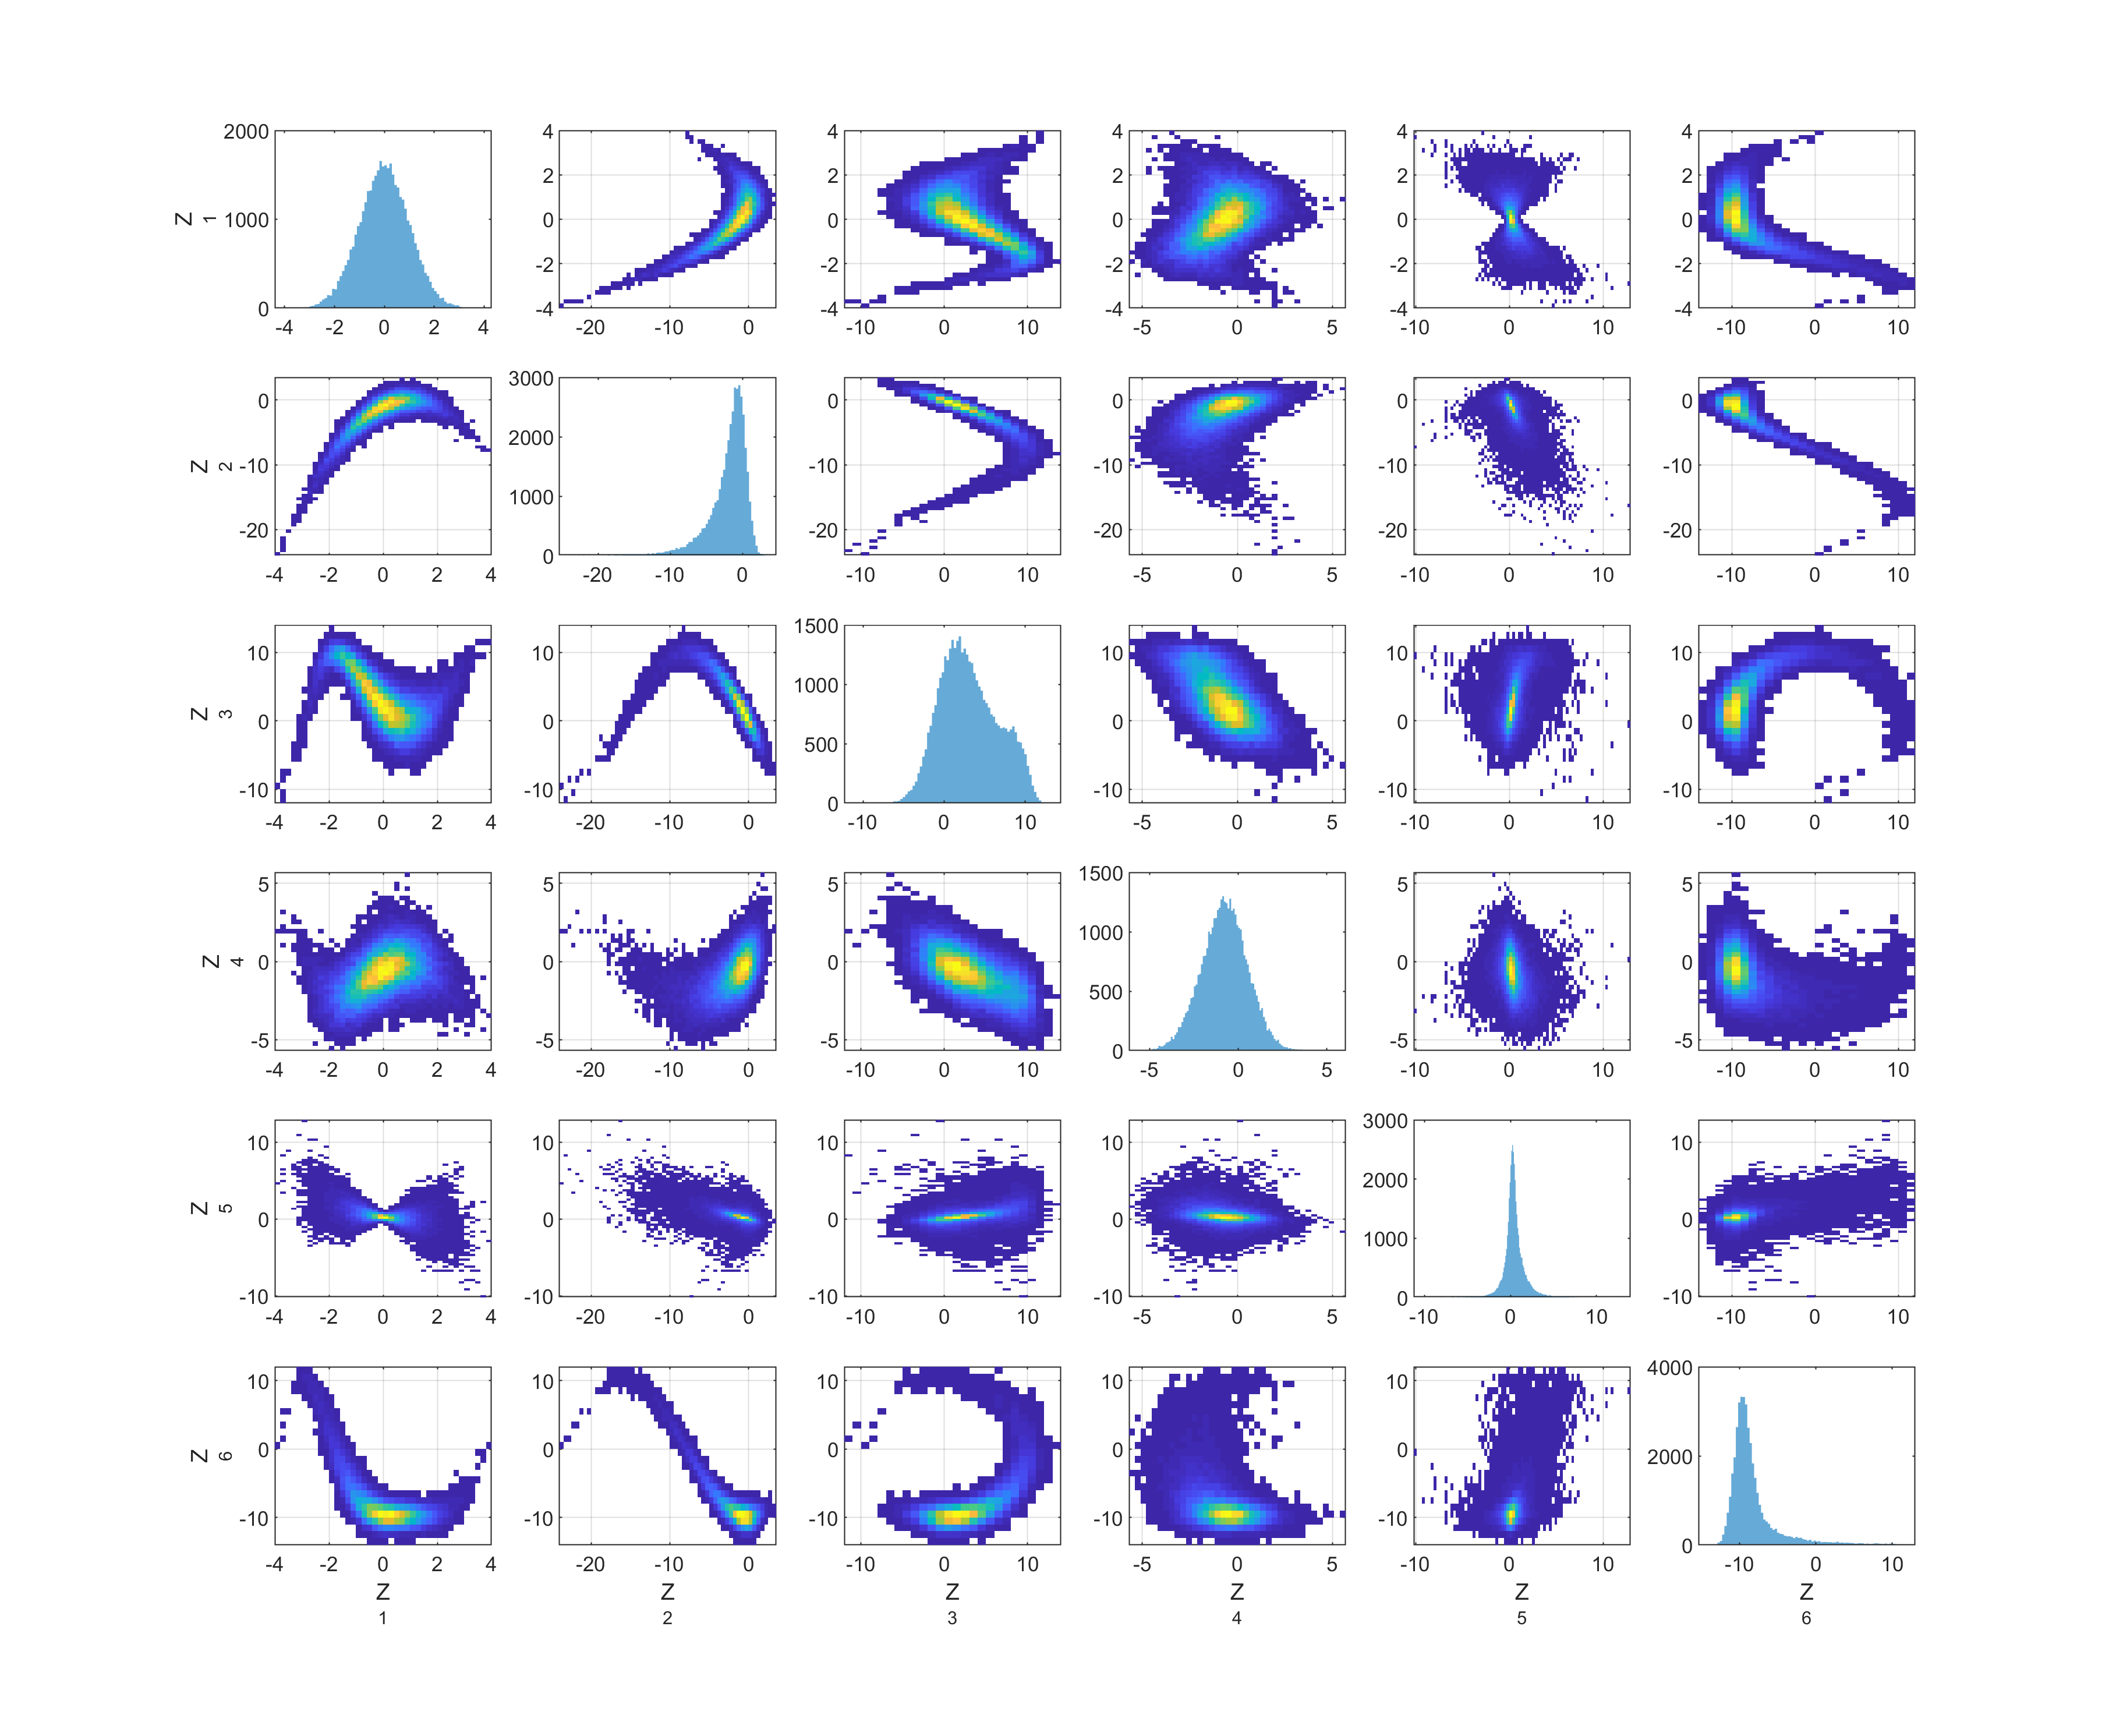
\includegraphics[width=0.75\textwidth]{figs_rev1/uncond_distribution_reference.png}
\caption{ Caption here. Image from \cite{de2021direct}.}
\label{fig:Figure1}
\end{figure}

This section includes an example of table (Table \ref{tab:Table1}).

\begin{table}
\centering
\caption{Example of table.}
\label{tab:Table1}
\begin{tabular}{ |c||c|c|c|} 
 \hline
     & $a$  &  $b$  &  $c$\\ 
 \hline 
 \hline
$a$ & 0.014 &  0.20    &   0.13  \\
\hline
$b$ & 0.20    &   0.17    &   2.46    \\
\hline
$c$ & 0.13    &   2.5     &   0.31   \\
\hline
\end{tabular} 
\end{table}


\subsection{Subsection}

Text ...

\section{Conclusions}

Conclusions here...

\section{Acknowledgments}

The authors would like to acknowledge ...

\newpage

\textbf{Code availability section}

Name of the code/library

Contact: e-mail and phone number

Hardware requirements: ...

Program language: ...
 
Software required: ...

Program size: ...

The source codes are available for downloading at the link:
https://github.com/ . . . . 


\bibliographystyle{cas-model2-names}
\bibliography{bibliography} 

\end{document}

